\documentclass[nohyperref]{article}

\usepackage{microtype}
\usepackage{graphicx}
\usepackage{subfigure}
\usepackage{booktabs}
\usepackage{amsmath,amssymb,mathtools}
\usepackage{array}
\usepackage{enumitem}
\usepackage{xcolor}
\usepackage{listings}
\usepackage{placeins}
\usepackage{fontspec}
\usepackage[unicode,colorlinks=true,linkcolor=blue,citecolor=blue,urlcolor=blue]{hyperref}
\usepackage[accepted]{icml2022}

\setmainfont{Noto Serif CJK SC}
\setsansfont{Noto Sans CJK SC}
\setmonofont{Noto Sans Mono CJK SC}
\XeTeXlinebreaklocale "zh"
\XeTeXlinebreakskip = 0pt plus 1pt

\providecommand{\theHalgorithm}{\arabic{algorithm}}
\DeclareRobustCommand{\code}[1]{\texttt{\detokenize{#1}}}
\newcommand{\todoedit}[1]{\textcolor{red}{#1}}
\setcounter{topnumber}{3}
\setcounter{bottomnumber}{2}
\setcounter{totalnumber}{5}
\setcounter{dbltopnumber}{3}
\renewcommand{\topfraction}{0.95}
\renewcommand{\bottomfraction}{0.85}
\renewcommand{\textfraction}{0.05}
\renewcommand{\floatpagefraction}{0.80}
\renewcommand{\dbltopfraction}{0.95}
\renewcommand{\dblfloatpagefraction}{0.80}
\setlength{\textfloatsep}{7pt plus 2pt minus 2pt}
\setlength{\floatsep}{7pt plus 2pt minus 2pt}
\setlength{\intextsep}{7pt plus 2pt minus 2pt}
\setlength{\dbltextfloatsep}{9pt plus 2pt minus 2pt}

\lstset{
  basicstyle=\ttfamily\scriptsize,
  breaklines=true,
  columns=fullflexible,
  frame=single,
  backgroundcolor=\color{gray!6},
  rulecolor=\color{gray!30},
  xleftmargin=0.5em,
  xrightmargin=0.5em,
  showstringspaces=false
}

\icmltitlerunning{\smash{MARL Sokoban}}

\begin{document}

\twocolumn[
\icmltitle{双人合作推箱子环境中的多智能体强化学习探索\\
基于 HARL 的 HAPPO、Reward Shaping、输入模式与信用分配实验}

\begin{icmlauthorlist}
\icmlauthor{石彦博}{}
\icmlauthor{陈龙}{}
\end{icmlauthorlist}

\icmlkeywords{Multi-Agent Reinforcement Learning, Sokoban, HAPPO, Reward Shaping, Credit Assignment}
\vskip 0.3in
]


\begin{abstract}
本报告围绕课程组队课题中的``2人合作推箱子''任务，整理了我们在 \code{gym-sokoban} 与 HARL 框架上的环境接入、模型结构、奖励塑形、输入历史、信用分配与算法改动探索。我们将原始双人 Sokoban 封装为 HARL 标准多智能体接口，采用 turn-based 动作执行与 action mask，主线使用 HAPPO 训练。实验显示：在固定 7x7、2 箱子的设置下，HAPPO 能够稳定学习，其中去除 deadlock 与 pushability 负项的 \code{v1-nodl-nopush} 是当前实现中最稳的 baseline；更符合推箱语义的 reverse-push reward shaping v2 并未带来更高成功率，更精确的奖励反而使优化更崎岖，而不可达距离的 cap 对控制信号尺度十分关键；模型架构上 GRU 表现最好，显式输入动作历史会降低 GRU 性能，\code{mlp-8} 也劣于 \code{gru-8}，这说明历史输入虽能在原理上把非 Markov 环境 Markov 化，但``可表示''不等于``易优化''；引入 GRPO-style 相对优势的 HAHyPO 没有带来性能提升，其轨迹级相对排序信号过粗，难以替代逐步 advantage；信用分配是核心问题，但当前 actor-side credit 收益有限；在 13x13 padding 上，random padding 几乎无法训练，top-left padding 虽仍困难但 CNN 明显最优，体现了空间归纳偏置与平移不变性的价值，distillation 则受限于模型容量而未见效果。最终提交模型为不显式输入动作历史的 GRU 版本 \code{GRU0}。
\end{abstract}

\section{任务与要求}
课程要求在双人 Sokoban 环境中控制两个智能体（环境来自 gym-sokoban~\citep{schrader2018sokoban}），将箱子推到目标位置。作业关注完整训练评估流程、算法设计、创新探索、训练参数、核心代码、实验曲线和结果分析。给定基准 HARL 框架~\citep{harlrepo} ，我们采用其中的 HAPPO~\citep{kuba2021trust} 作为baseline；环境原始奖励为团队共享奖励，可以考虑信用分配。

我们选择 \code{TwoPlayer-Sokoban-v0} 作为主环境，并尝试扩展到 \code{v0/v1/v2} 混合训练。主要目标是系统比较以下方向：
\begin{itemize}[leftmargin=1.2em,itemsep=0.2em]
    \item 模型结构：MLP、CNN、GRU/RNN 以及动作历史输入。
    \item 奖励塑形：原始奖励、旧 BFS 势函数、reverse-push v2、deadlock/pushability 消融。
    \item 信用分配：共享团队回报、active-agent mask、actor-side credit 辅助项。
    \item 算法探索：HAPPO 主线、actor-side credit 与 HAHyPO 混合优势函数。
\end{itemize}

\section{Settings}

原始双人 Sokoban 环境底层仍是一个 gym 环境。我们在 \path{HARL/harl/envs/sokoban/sokoban_env.py} 中将其封装成 HARL 所需接口。

\subsection{Action Modeling}
每个 agent 输出一个 \code{Discrete(9)} 动作，分别表示 \code{noop}+四个方向移动+四个方向推箱子。采用 turn-based 建模：每步只有当前 active agent 可以选择非 \code{noop} 动作，另一个 agent 的 action mask 中只有 \code{noop} 可用。显然，任给一个同步动作$ (a_1, a_2)$ 可以拆分成两个合理的异步行动$ (a_1, noop)$, $ (noop, a_2)$；任给异步轮换行动序列也可以转化成同步行动策略，故在可表示性上二者没有差别。由于我们mask掉所有其他action，对另一个不动的agent写策略梯度，$\nabla log\pi (a|s)$ 项由于$\pi (a|s)$恒为1而恒等于0，对更新没有任何影响。

\begin{lstlisting}[language=Python,caption={Turn-based 动作解析的核心逻辑。}]
def _resolve_action(self, actions):
    chosen_agent = self._priority_agent
    chosen_action = actions[chosen_agent]
    invalid_action_attempt = any(
        actions[i] != 0 for i in range(self.n_agents)
        if i != chosen_agent
    )
    if chosen_action == 0:
        return chosen_agent, 0, info
    if chosen_agent == 0:
        return chosen_agent, chosen_action, info
    return chosen_agent, chosen_action + 8, info
\end{lstlisting}

\begin{figure*}[!t]
\centering
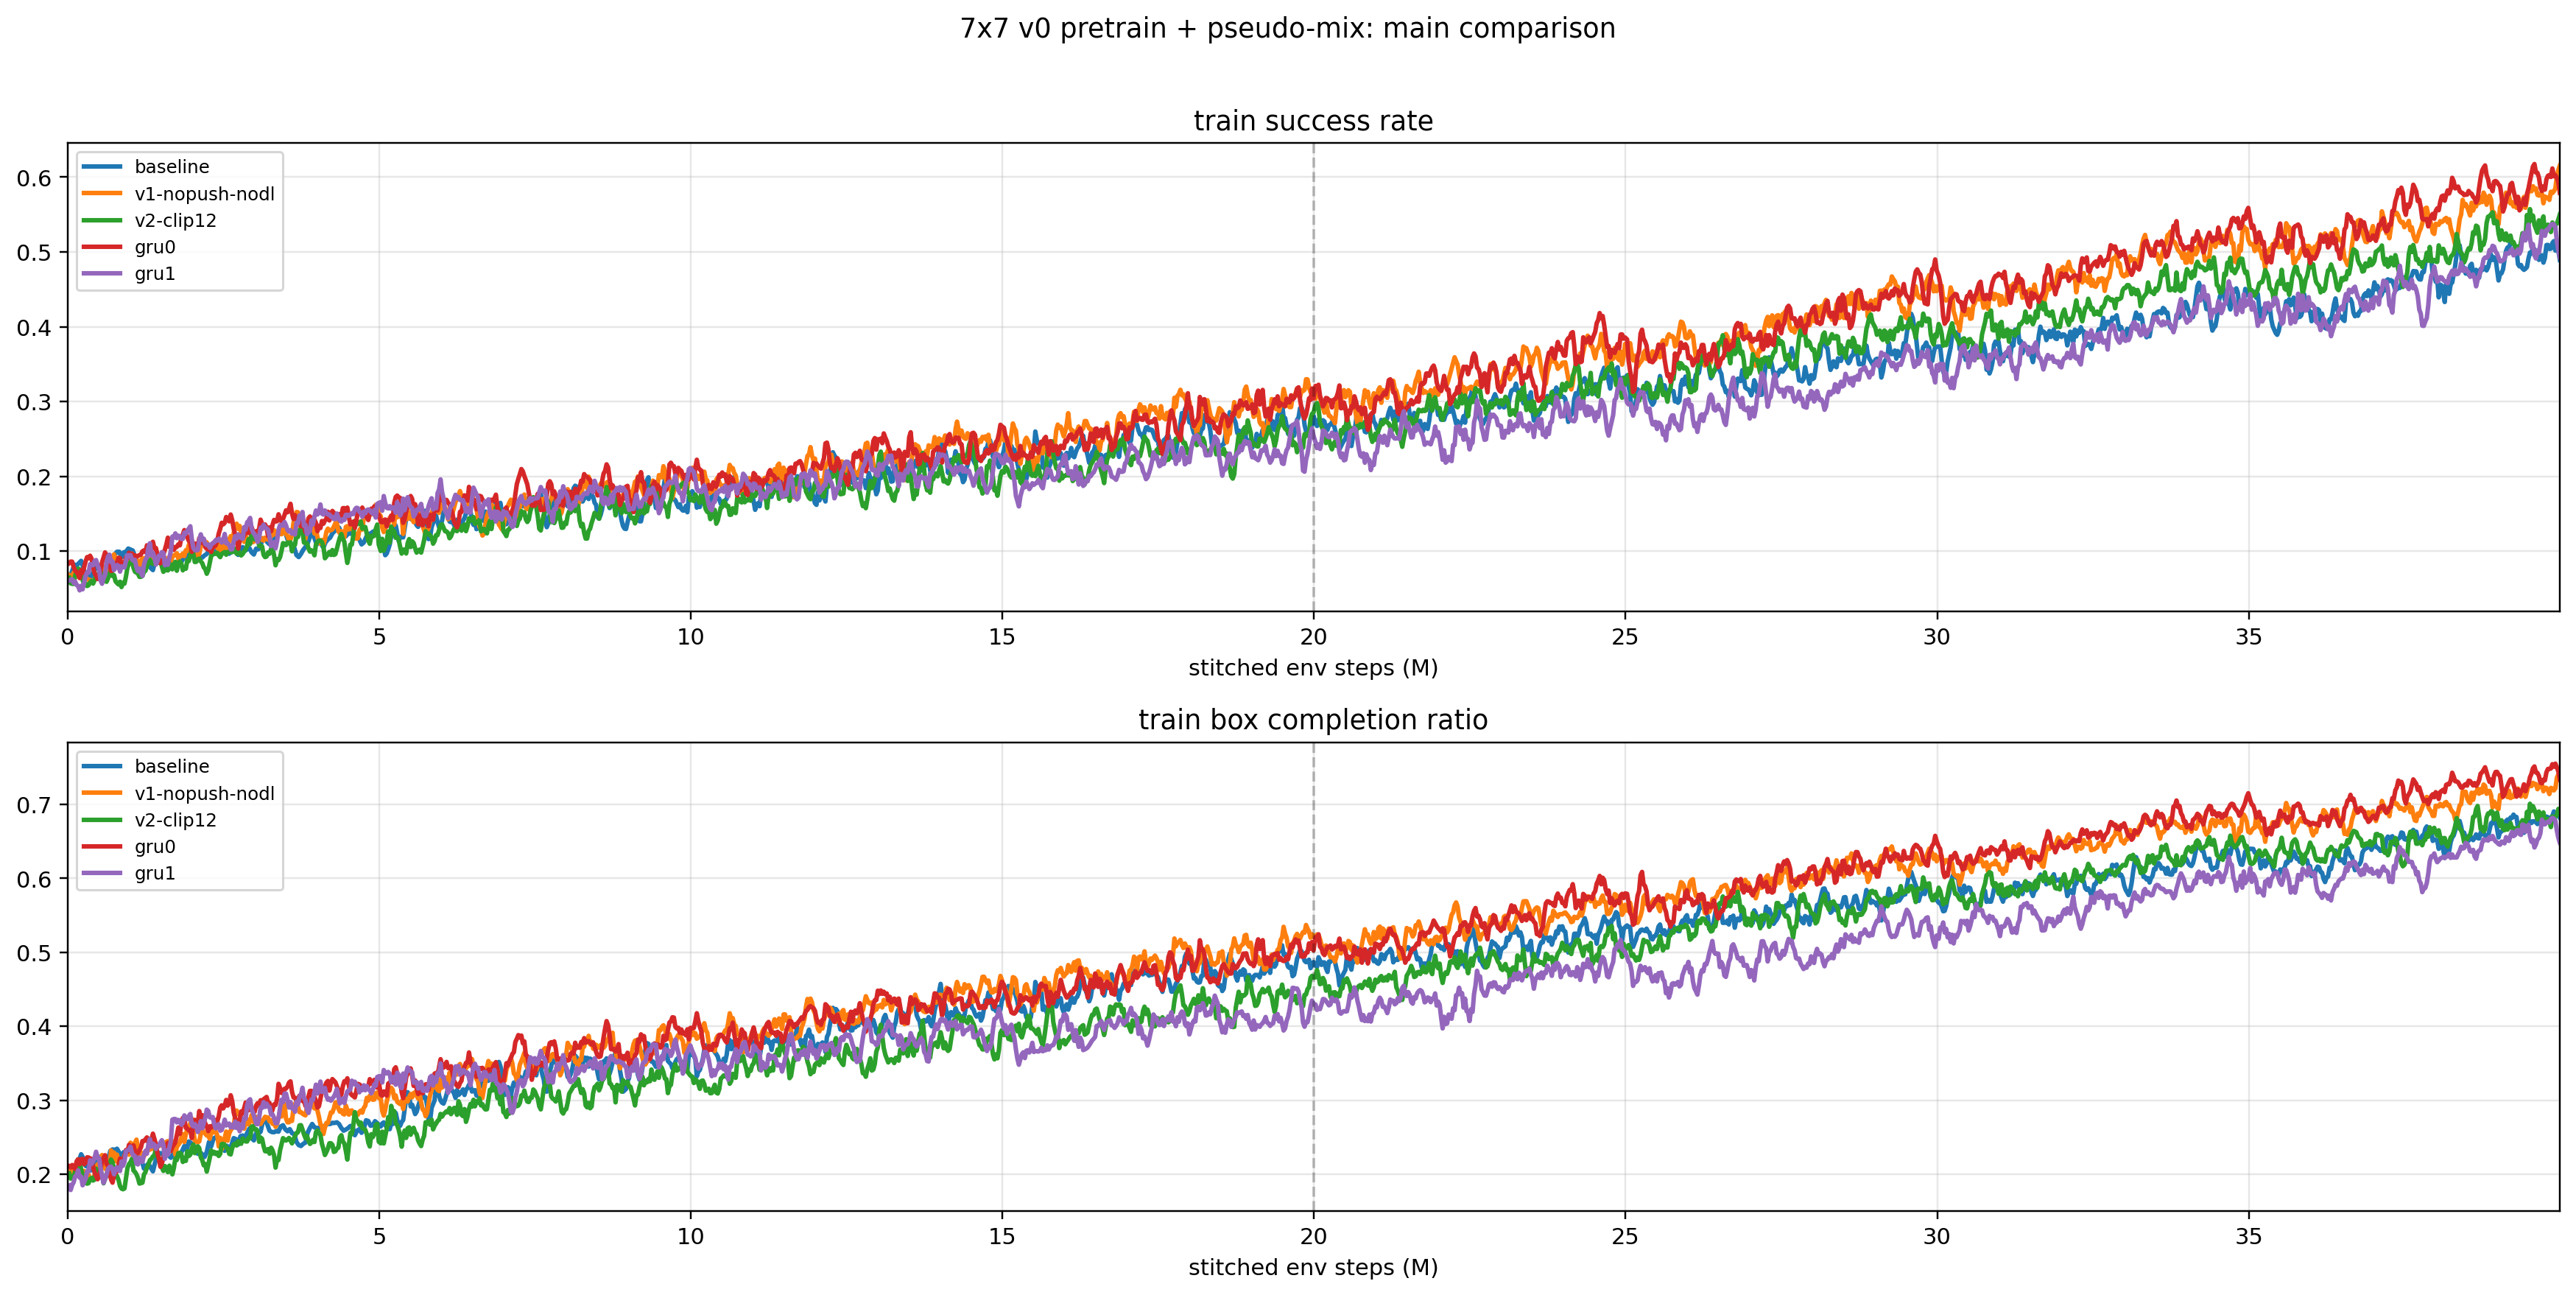
\includegraphics[width=0.95\textwidth]{figures/fig1_main_train_success_box_ratio.png}
\caption{7x7、2 boxes 固定环境下的主线长跑结果，比较 HAPPO baseline 与若干轻量塑形/架构变体。曲线显示各方案均能脱离随机策略并持续上升；其中去掉 deadlock 与 pushability 负项的 \code{v1-nodl-nopush} 收敛最稳、波动最小，是当前实现中最稳的 baseline。}
\label{fig:old7x7}
\end{figure*}

这种封装有两个好处。第一，它避免两个 agent 在同一步同时改变底层环境导致冲突裁决噪声，这是符合HARL的设计思路的。第二，inactive agent 的 actor 不会因为不可执行动作被错误训练，后续 credit assignment 也更容易定义。

\subsection{Agent Observation}
默认观测为符号化向量。每个 agent 看到墙、目标、目标上的箱子、普通箱子、自己位置、队友位置六类二值图，并额外拼接当前 active agent 标志与步数比例。共享状态使用同样的全局符号图。为比较模型结构，我们同时支持 CNN 输入：将上述通道堆叠为 channel-first 图像，并使用三层小型 Sokoban CNN encoder。为研究部分可观测性与轮流执行记忆，环境还支持 \code{action_history_len=K}，将过去 $K$ 步实际执行的联合动作 one-hot 拼接到 observation 或作为常数通道加入 CNN observation。

\subsection{Padded Observation in Concern of Compatibility}
虽然我们的主实验采用的是\code{scenario_pool=v0} 环境，即\code{dim_room=7,num_boxes=2} ，但我们尝试将模型扩展到更复杂的环境下完成训练。对于基础的MLP模型等，网络维度很显然与观测视野的大小有关，为处理不同环境的观测视野不同的问题，我们增设固定观测画布：
\begin{itemize}[leftmargin=1.2em,itemsep=0.2em]
    \item \code{use_mixed_obs_padding=True}，\code{obs_dim_room=13}；
    \item padding 模式包括 \code{random_episode}、\code{top_left}；
    \item 让 \code{v0/v1/v2} 保留原始复杂度差异。
\end{itemize}
这使网络输入维度固定，显著增加了在各种环境的兼容性；然而这实际上会显著增大训练的难度，这将在5.5中详细论述。



\section{Methods}

sokoban游戏的目标是两个智能体合力将箱子推到目标位置，所有优化围绕着最终目标进行。在后文中，箱子也称为box，智能体也称为agent，目标位置也称为target。推箱子进行的环境被称为地图。定义地图中两个位置之间的距离为曼哈顿距离（同时也是L1距离）。又定义两个位置之间的BFS距离为限制条件下的曼哈顿距离（数值上等价于：如果图中有某些点是不可达的，从一个位置到另一个位置至少需要走的步数）。

\subsection{HAPPO Baseline}
主线采用 HAPPO。HAPPO \cite{kuba2021trust} 继承 PPO 的 clipped policy optimization 思路~\citep{schulman2017proximal}，使用中心化 critic 和分 agent actor，critic 学习共享团队回报，actor 按顺序更新并用重要性因子修正已经更新过的 agent 对联合策略的影响。训练参数见表 \ref{tab:params}。

\begin{table*}[t]
\caption{主线训练参数。不同脚本会对模型或 reward 做小幅改动，但多数长跑实验共享该设置。}
\label{tab:params}
\centering
\small
\begin{tabular}{p{0.13\textwidth}p{0.80\textwidth}}
\toprule
项目 & 设置 \\
\midrule
环境 & \code{TwoPlayer-Sokoban-v0}，7x7，2 boxes，\code{max_steps=150}；真 mix 使用 \code{v0/v1/v2} + 13x13 padding \\
并行采样 & 7x7 MLP 常用 \code{n_rollout_threads=32},部分GRU模型为加速训练采用\code{n_rollout_threads=48} \\
训练阶段 & 每阶段 5M steps，完整长程实验采用8阶段训练 \\
优化器 & \code{lr=1e-4}，\code{critic_lr=3e-4}，\code{ppo_epoch=5}，\code{clip_param=0.1} \\
网络 & MLP \code{[512,512]}；CNN \code{[32,64,64]} 三层卷积；GRU \code{recurrent_n=1,data_chunk_length=25} \\
\bottomrule
\end{tabular}
\end{table*}


\subsection{Reward Shaping}
原始环境奖励为：每步 $-0.1$，箱子推上目标 $+1$，箱子离开目标 $-1$，全部完成 $+10$。首先，$+10$的终局奖励看起来过于稀少，对智能体的激励幅度有限，着眼于此我们将终局奖励提升到 $+20$。但由于终局奖励仍然过于稀疏，早期随机策略很难稳定发现箱子和将箱子推到目标的获利方法。我们在 \path{HARL/harl/envs/sokoban/reward_shaping.py} 中实现了可开关的 reward shaping。它不改变任务目标，只把 Sokoban 中较明确的进展转成低方差的中间学习信号。

\subsubsection{Distance Potentials: Box-Target and Agent-Box}
距离塑形分成两类势函数。第一类是 box-target distance $D_{bt}(s)$，衡量所有箱子到所有target的最小匹配距离；第二类是 agent-box distance $D_{ab}(s)$，衡量两名 agent 到有用推箱站位或箱子相邻格的距离。每一步使用势函数差分：如果动作让箱子更接近目标，或让 agent 更接近可执行推箱的位置，就得到正奖励；反之得到负或零奖励。

我们实现了两种距离语义。\textbf{方案一（v1）} 使用朴素 BFS。具体来说，box-target distance定义为只有墙限制下所有箱子与所有目标最小匹配BFS距离，这是理论可行的最短距离。任意两个agent和box之间的距离定义考虑墙、箱子和另一智能体限制下，agent到箱子相邻空余位置的最短 BFS 距离，由此出发定义势函数
$$D_{ab}(s) = 
\sum_{box} \left[ 
\min_{a,\, \text{与box相邻的任意}c} 
\big( \text{dist}_{\text{BFS}}(a, c) + 1 \big) 
\right]
$$
方案1的距离比较粗糙，但 reward 尺度稳定、噪声小，是后来表现最稳的主线。

\textbf{方案2（v2）} 使用 reverse-push distance，出发点来源于对v1的修正。显然，箱子要想移动，必须提供相邻格子处一个空位供agent站立，且在箱子被推向的方向上有移动空间。box-target的具体实现为从目标反向搜索箱子位置，同时检查``箱子前一格''和``玩家站位格''都不是墙，在此条件下的最优匹配；agent-box 也不再奖励靠近任意箱子，而是奖励靠近那些推动后能降低全局 box-target distance 的 useful rear cells。该方法更符合语义，但不可达状态会产生更大的距离跳变，对于在尝试中箱子被推到死角惩罚过重，在实验中我们发现使用该奖励很容易导致智能体趋向于不动。因此，需要用 \code{shaping_unreachable_distance=12} 一类裁剪控制尺度，避免不可达时过重惩罚。

实际 reward 使用前后状态差分：
\begin{align}
 r^{dist}_t &= w_{bt}\Delta D_{bt,t}
              + w_{ab}\Delta D_{ab,t}, \\
 \Delta D_{\bullet,t} &= D_{\bullet}(s_t)-D_{\bullet}(s_{t+1}).
\end{align}
距离绝对值只影响势函数尺度，真正奖励的是动作带来的相对进展。

\subsubsection{Penalties: Deadlock, Pushability and Useless Actions}
除距离进展外，我们还探索了若干惩罚项。

第一，\textbf{死锁惩罚（deadlock）}。死锁用于描述这样一种现象：箱子被推到角落，此时箱子无法再被推动。其形式化定义是箱子的可移动方向的补集与空闲站位的集合无交。Deadlock $L(s)$ 统计非目标格上、当前完全不可推动的箱子，只在死锁箱数量增加时施加权重为$\lambda_{dl}$的惩罚，避免同一坏状态每步重复重罚导致智能体失去探索热情。

第二，\textbf{自由度惩罚（pushability）}。Pushability $P(s)$ 是所有箱子当前可推动方向数的总和；如果一步动作让可推动方向减少，就给负奖励。事实上这是对死锁惩罚的扩展，可以理解为广义deadlock penalty。

\begin{lstlisting}[language=Python,caption={自由度惩罚的伪代码计算.}]
def box_pushability(state, box):
    k = 0
    reachable = cells_reachable_by_any_agent(
        blocked = walls | boxes | other_agents
    )

    for d in directions:
        front = box + d      # cell the box moves into
        rear  = box - d      # cell where an agent must stand

        if front in walls or front in boxes or front in agents:
            continue
        if rear not in reachable:
            continue

        k += 1

    return k

def pushability_potential(state):
    return sum(box_pushability(state, b) for b in boxes)
\end{lstlisting}

第三，\textbf{动作不合法惩罚（illegal actions）}。其核心想法是：如果 agent 输出的动作在当前局面下显然不可能产生有效变化，就额外给 $\lambda_{useless}$的小惩罚。例如：agent 没碰到箱子却选择某个 push 动作；agent 离所有箱子较远时选择 \code{noop}；agent 选择移动但该方向是墙，导致位置不变。这类 penalty 可作为稀疏任务中的行为先验，帮助策略少浪费 rollout budget。


\subsubsection{Total Reward and Common Parameters}
综合上述项，我们使用的总 reward 可以写成：
\begin{align}
 r_t =&\ r_t^{base}
 + w_{bt}\Delta D_{bt,t}
 + w_{ab}\Delta D_{ab,t} \notag\\
 &+ w_p \min(0, \Delta P_t)
 - \lambda_{dl}\max(0,\Delta L_t) \notag\\
 &- \lambda_{inv} I^{inv}_t
 - \lambda_{useless} I^{useless}_t,
\end{align}
其中 $\Delta P_t=P_{t+1}-P_t$，$\Delta L_t=L_{t+1}-L_t$；$I^{inv}_t$ 表示非法 push 或撞墙移动，$I^{useless}_t$ 表示远离箱子时 \code{noop} 或动作后状态无变化。主线 \code{v1-nodl-nopush} 使用 v1 的距离势函数，参数为 $w_{bt}=0.20$、$w_{ab}=0.10$、$w_p=0$、$\lambda_{dl}=0$，并使用 \code{reward_finished=20}。v1 额外使用 $w_p=0.05$ 和 $\lambda_{dl}=0.8$；v2-clip12 使用 \code{reverse_push/useful} 距离并设置 unreachable distance cap 为 12。

\subsection{信用分配与 Actor-Side Credit}
turn-based 机制下每步只有 active agent 真实影响环境，而环境奖励仍是团队共享，因此信用分配在本任务中是真实存在的问题。我们做了两层处理：active mask 保证 inactive agent 只有 \code{noop} 可选、其 actor buffer 中 active mask 为 0；在此基础上尝试 actor-side credit，即 critic 仍学习团队 reward，只在 active agent 的优势函数上叠加一个小型辅助信用项。

\begin{lstlisting}[language=Python,caption={Actor-side credit 只改变 active actor 的优势函数，不改变 critic 目标。}]
if mode == "active_progress":
    credit = max(base_reward, 0.0)
    credit += max(useful_push_distance_delta, 0.0)
    credit += max(agent_box_distance_shaping_reward, 0.0)
    if action_moved_box:
        credit += 0.2
A_actor = A_team + coef * credit
\end{lstlisting}

需要说明的是，actor-side credit 目前并未给出决定性提升（见第 \ref{sec:credit} 节）：active mask 是必要基础，而额外的 actor 信用项更多是探索性尝试。

\subsection{HAHyPO 与 GRPO-Style Advantage}
除 HAPPO 外，我们实现了 HAHyPO 入口作为探索性变体。它保留 HAPPO 的 critic、GAE 与 clipped update，只改变 actor 使用的优势函数。动机来自 GRPO（Group Relative Policy Optimization）~\citep{shao2024deepseekmath}：GRPO 不依赖单独的 value model，而是在同一组样本内部用回报的相对高低构造优势。我们的 Sokoban 设置没有 prompt，但每次 rollout update 中存在多个并行环境轨迹，因此可以把同一 batch 内的 episode return 看成一个 group。记第 $i$ 条轨迹回报为 $R_i$，则 GRPO-style trajectory advantage 为：
\begin{equation}
 A^{GRPO}_i=\frac{R_i-\mathrm{mean}_j(R_j)}{\mathrm{std}_j(R_j)+\epsilon}.
\end{equation}
HAHyPO 使用混合优势：
\begin{equation}
A^{actor}=(1-\alpha)\,\mathrm{zscore}(A^{GAE})+
\alpha\,A^{GRPO}.
\end{equation}
其中 critic 仍学习正常团队回报，因此这是一个保守的 hybrid ablation，而非纯 GRPO。这一改动的重点不在于``实现了新的 actor 入口''，而在于它为什么没有比主线更好：实验显示（见第 \ref{sec:hahypo} 节）GRPO-style 项并未带来性能提升。这与语言模型中的使用场景不同——GRPO 的组内相对排序是轨迹级、较粗的信号，难以替代 Sokoban 这类稀疏、长时序、强 credit assignment 依赖任务所需的逐步优势估计。因此 HAHyPO 可作为探索性变体保留，但不构成对 HAPPO 主线的改进。

\begin{figure}[!tbp]
\centering
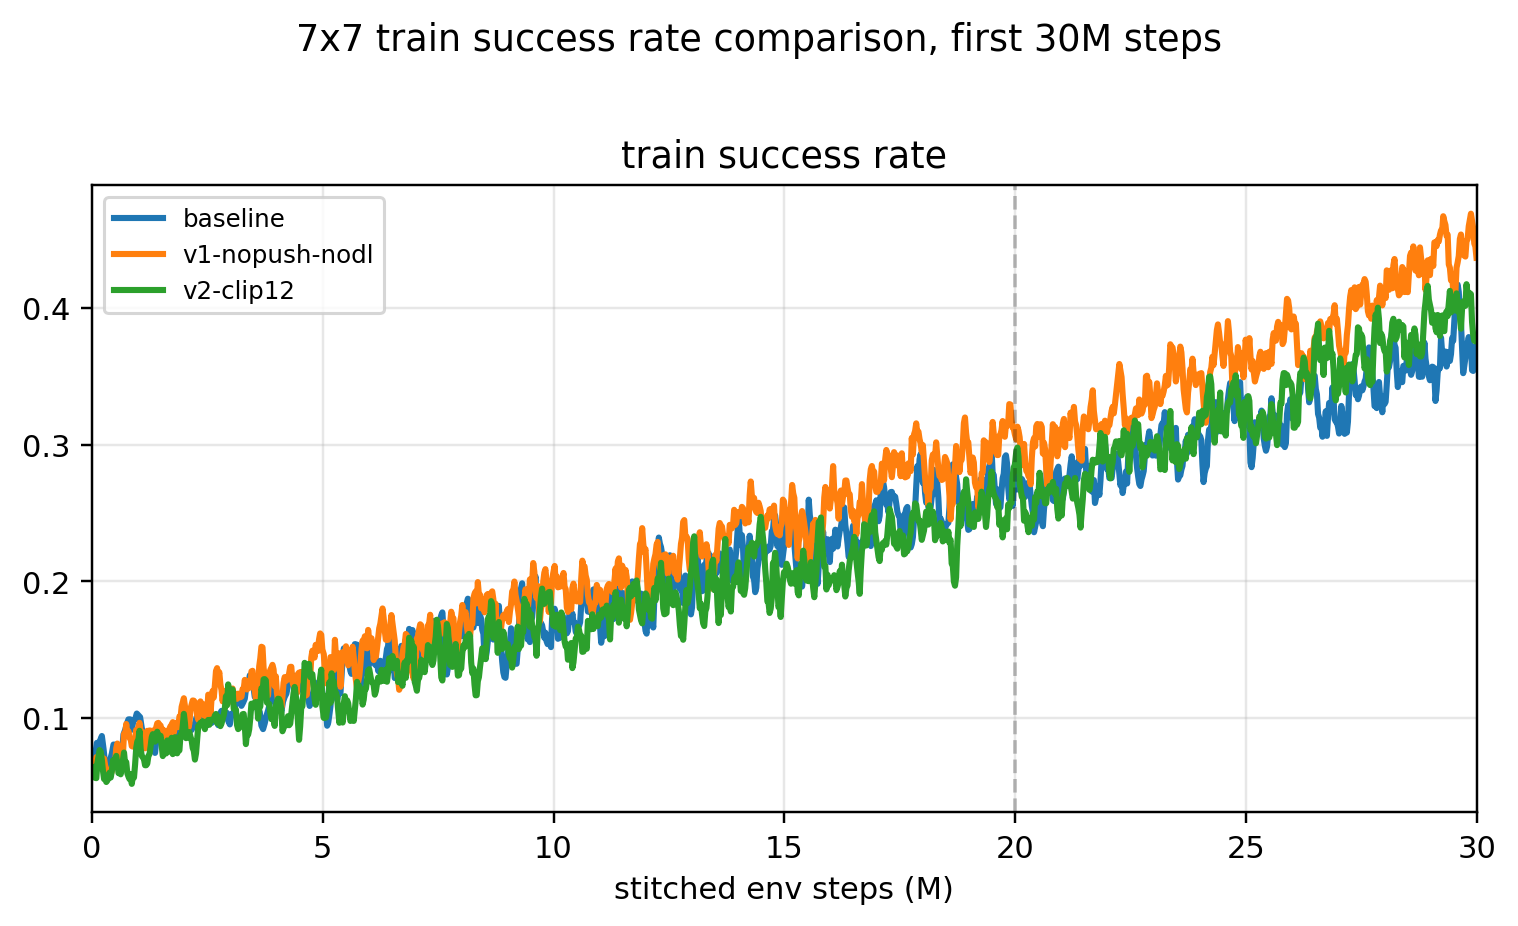
\includegraphics[width=\columnwidth]{figures/17_v2_clip12_baseline_v1_train_success_30m.png}
\caption{v2 reverse-push distance 与 v1、baseline 的长程比较。v2 在语义上更贴近真实推箱约束，clip12 后期有所追赶，但成功率仍未稳定超过旧 BFS 主线，说明语义更精确不必然更好学。}
\label{fig:v2cap}
\end{figure}

\begin{figure}[!tbp]
\centering
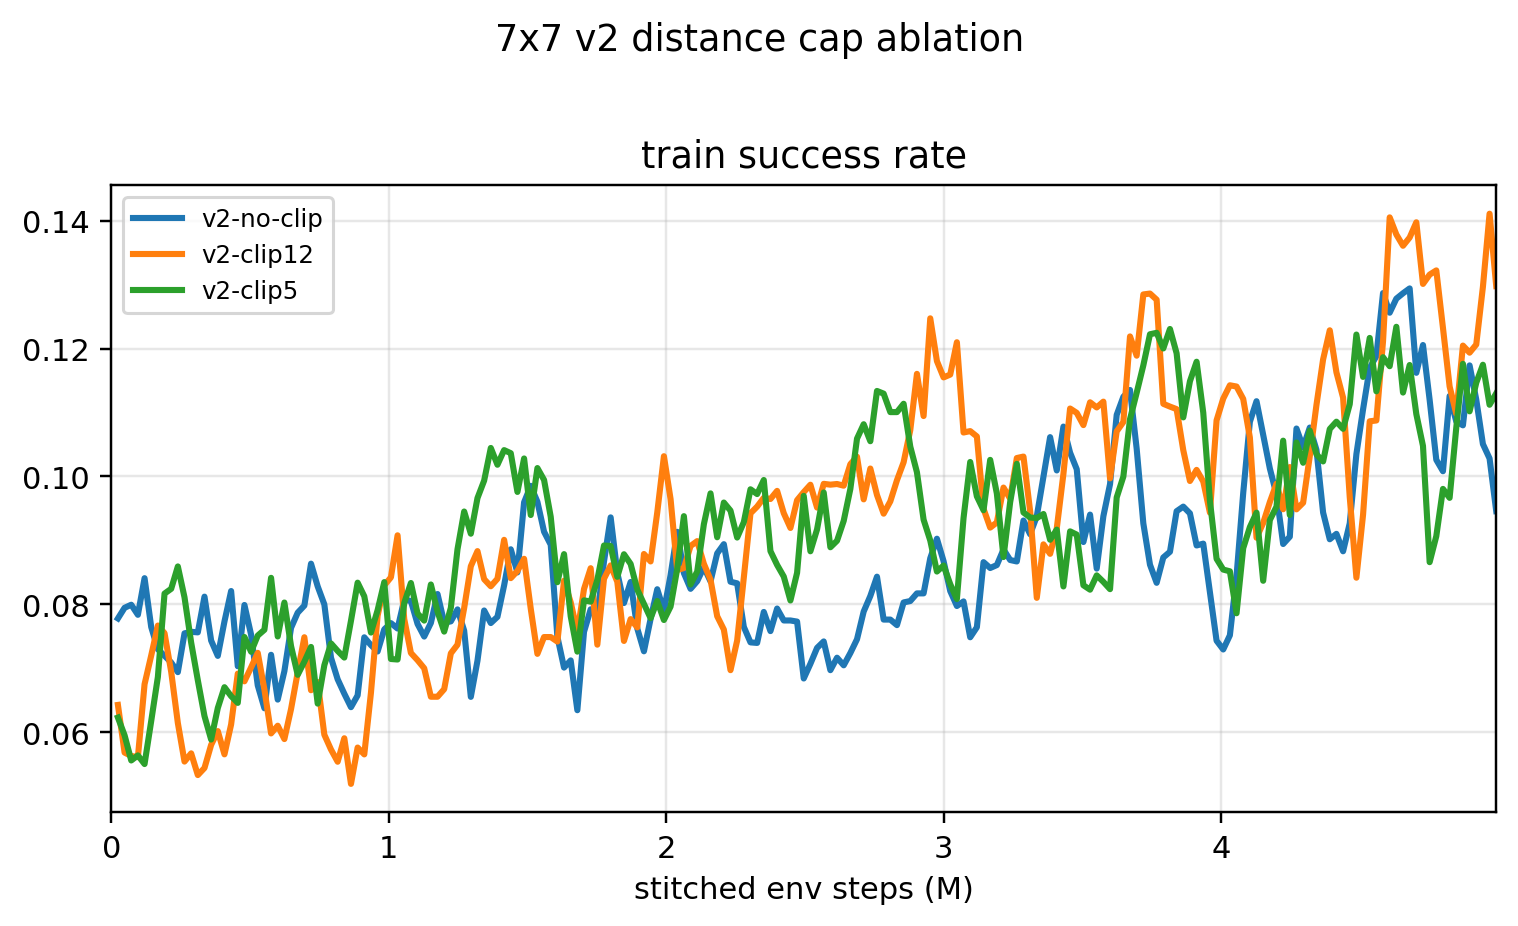
\includegraphics[width=\columnwidth]{figures/fig2_v2_success_ablation.png}
\caption{v2 reverse-push distance 的 unreachable-distance cap 消融。cap=12 在短程内表现最好，说明对不可达距离做裁剪、控制塑形信号尺度十分重要。}
\label{fig:v2clip}
\end{figure}

\begin{table*}[t]
\caption{主要实验系列与用途。}
\label{tab:runs}
\centering
\small
\begin{tabular}{p{0.12\textwidth}p{0.34\textwidth}p{0.43\textwidth}}
\toprule
系列 & 对应探索 & 主要结论用途 \\
\midrule
\code{run0} & 原始 reward baseline，长程 pretrain & 判断原始奖励是否可学，作为低 shaping 对照 \\
\code{run4--6} & CNN、旧 BFS reward shaping、deadlock/pushability 消融 & 得到 \code{v1-nodl-nopush} 主线 \\
\code{run7--10} & reward shaping v2、不可达距离 cap、长跑续训 & 比较语义更强的 reverse-push 与旧 BFS \\
\code{run9,11} & GRU/RNN 与动作历史 \code{0/1/2/8/16} & 检查历史动作是否提升部分可观测性 \\
\code{run12--15} & 13x13 padding、真 v0/v1/v2 mix、distillation & 分析固定尺寸训练到多尺寸泛化的困难 \\
\code{run16} & active-agent actor-side credit & 检查在不改环境目标下能否降低 actor 方差 \\
\code{run17} & HAHyPO 混合优势函数，$\alpha\in\{0.2,0.5,1.0\}$ & 算法层替代 HAPPO advantage 的探索入口 \\
\code{run18} & 无用动作 penalty，$\lambda\in\{0.1,0.2\}$ & 考察低层行为先验对早期探索与行为分布的影响 \\
\bottomrule
\end{tabular}
\end{table*}


\section{实验组织}
为便于阅读，正文只保留少数有明确解释价值的标签，如主线 baseline \code{v1-nodl-nopush}，以及 \code{GRU-0}、\code{GRU-8}、\code{CNN}、\code{v2-clip}、\code{top-left padding}、\code{random padding}、\code{distillation}。表 \ref{tab:runs} 按系列概括主要实验：architecture/history 系列比较模型结构与动作历史，mix/padding 系列研究 13x13 兼容画布下的泛化，HAHyPO 系列考察 GRPO-style 优势，credit 系列考察 actor-side 信用项。完整脚本入口与逐脚本说明保存在仓库各 \code{run*/README.md} 中，正文不再逐一展开。


\section{结果与分析}
\subsection{主结果}
图 \ref{fig:old7x7} 给出 7x7、2 boxes 固定环境下的主线长跑结果，比较对象集中在 HAPPO baseline 与 \code{v1-nodl-nopush}。结果表明，HAPPO 在该难度下可以明显脱离随机策略，训练成功率与 box completion ratio 在长程内持续上升。在所有轻量方案中，保留正向势函数、去掉 deadlock 与 pushability 负项的 \code{v1-nodl-nopush} 收敛最稳、波动最小。因此我们把 \code{v1-nodl-nopush} 作为当前实现中最稳的 baseline，并以它作为后续各项消融的统一参照。

\begin{figure}[!tbp]
\centering
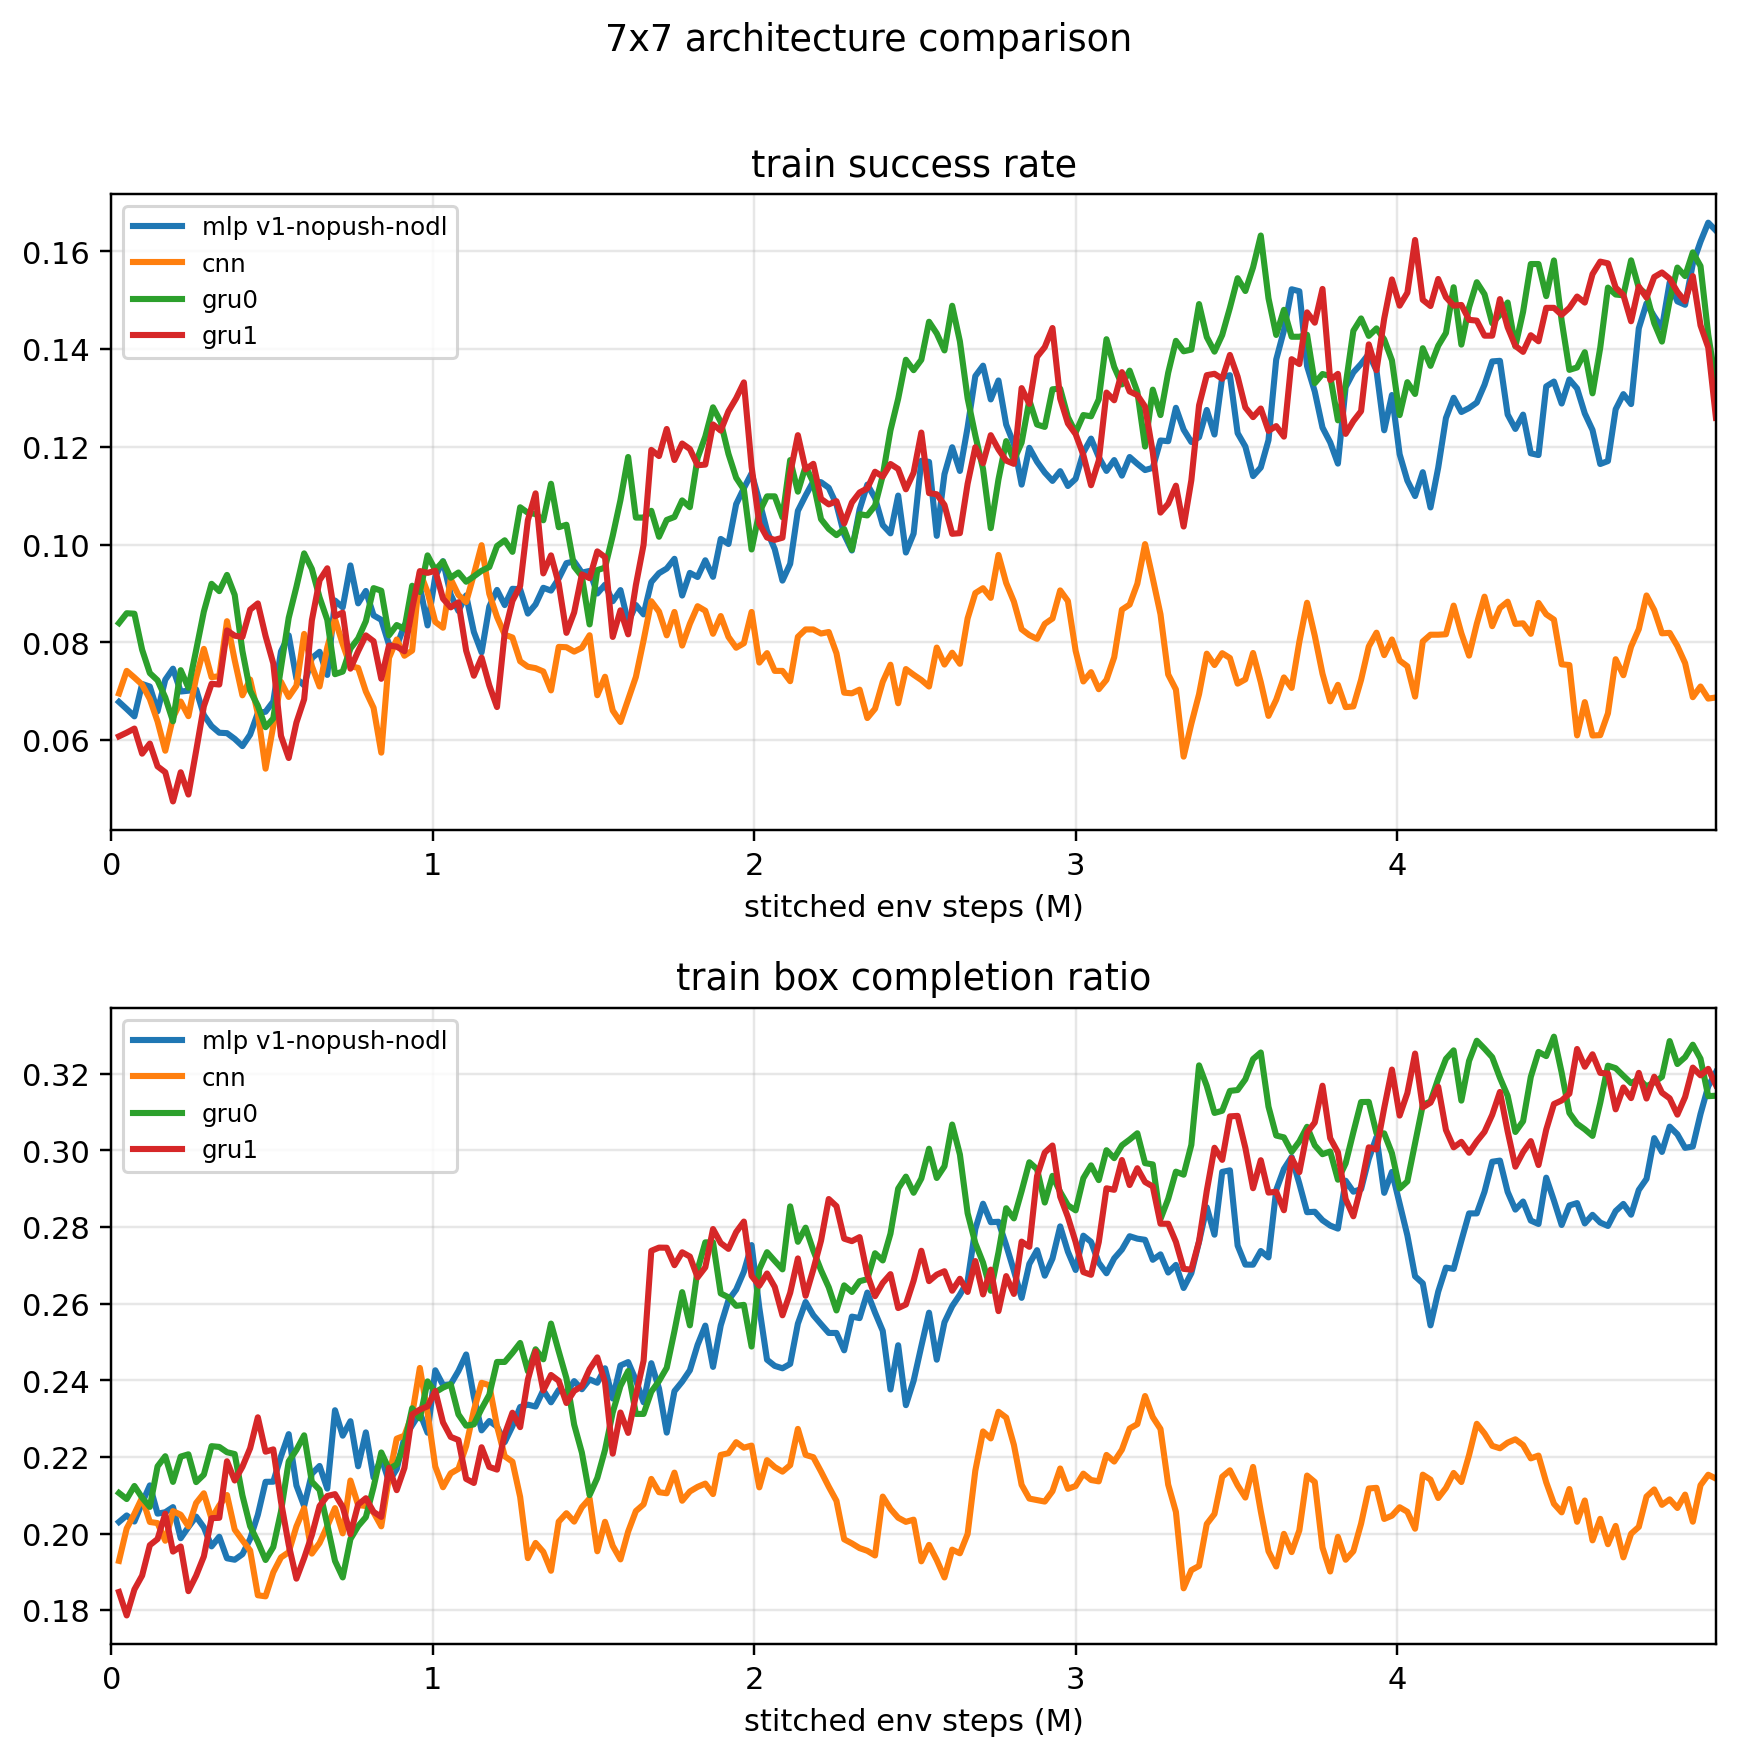
\includegraphics[width=\columnwidth]{figures/fig3_architecture_train_metrics.png}
\caption{7x7 模型结构比较。CNN 在小地图上不占优，GRU 的训练曲线更强；卷积的局部归纳偏置在小画布、稀疏回报、少通道符号输入下并未自动带来提升。}
\label{fig:arch7x7}
\end{figure}

\subsection{距离语义正确性的影响}
图 \ref{fig:v2cap} 与图 \ref{fig:v2clip} 比较了 v1 与 v2 reverse-push 距离。v2 在语义上更贴近``箱子能否被推到目标''的真实约束，但即使表现最好的 cap12 变体，在 7x7 长跑中也没有稳定超过 v1。结果显示，语义更精确不一定更好：更精确的 reward 会在不可达状态附近产生更大的距离跳变，使 optimization landscape 更崎岖，因此更难学。图 \ref{fig:v2clip} 的 cap 消融进一步说明，\code{v2-clip}/cap 很重要，因为它直接关系到塑形信号的尺度是否可控；缺少裁剪时，过重的不可达惩罚容易诱导 agent 趋向不动。

\begin{figure}[!tbp]
\centering
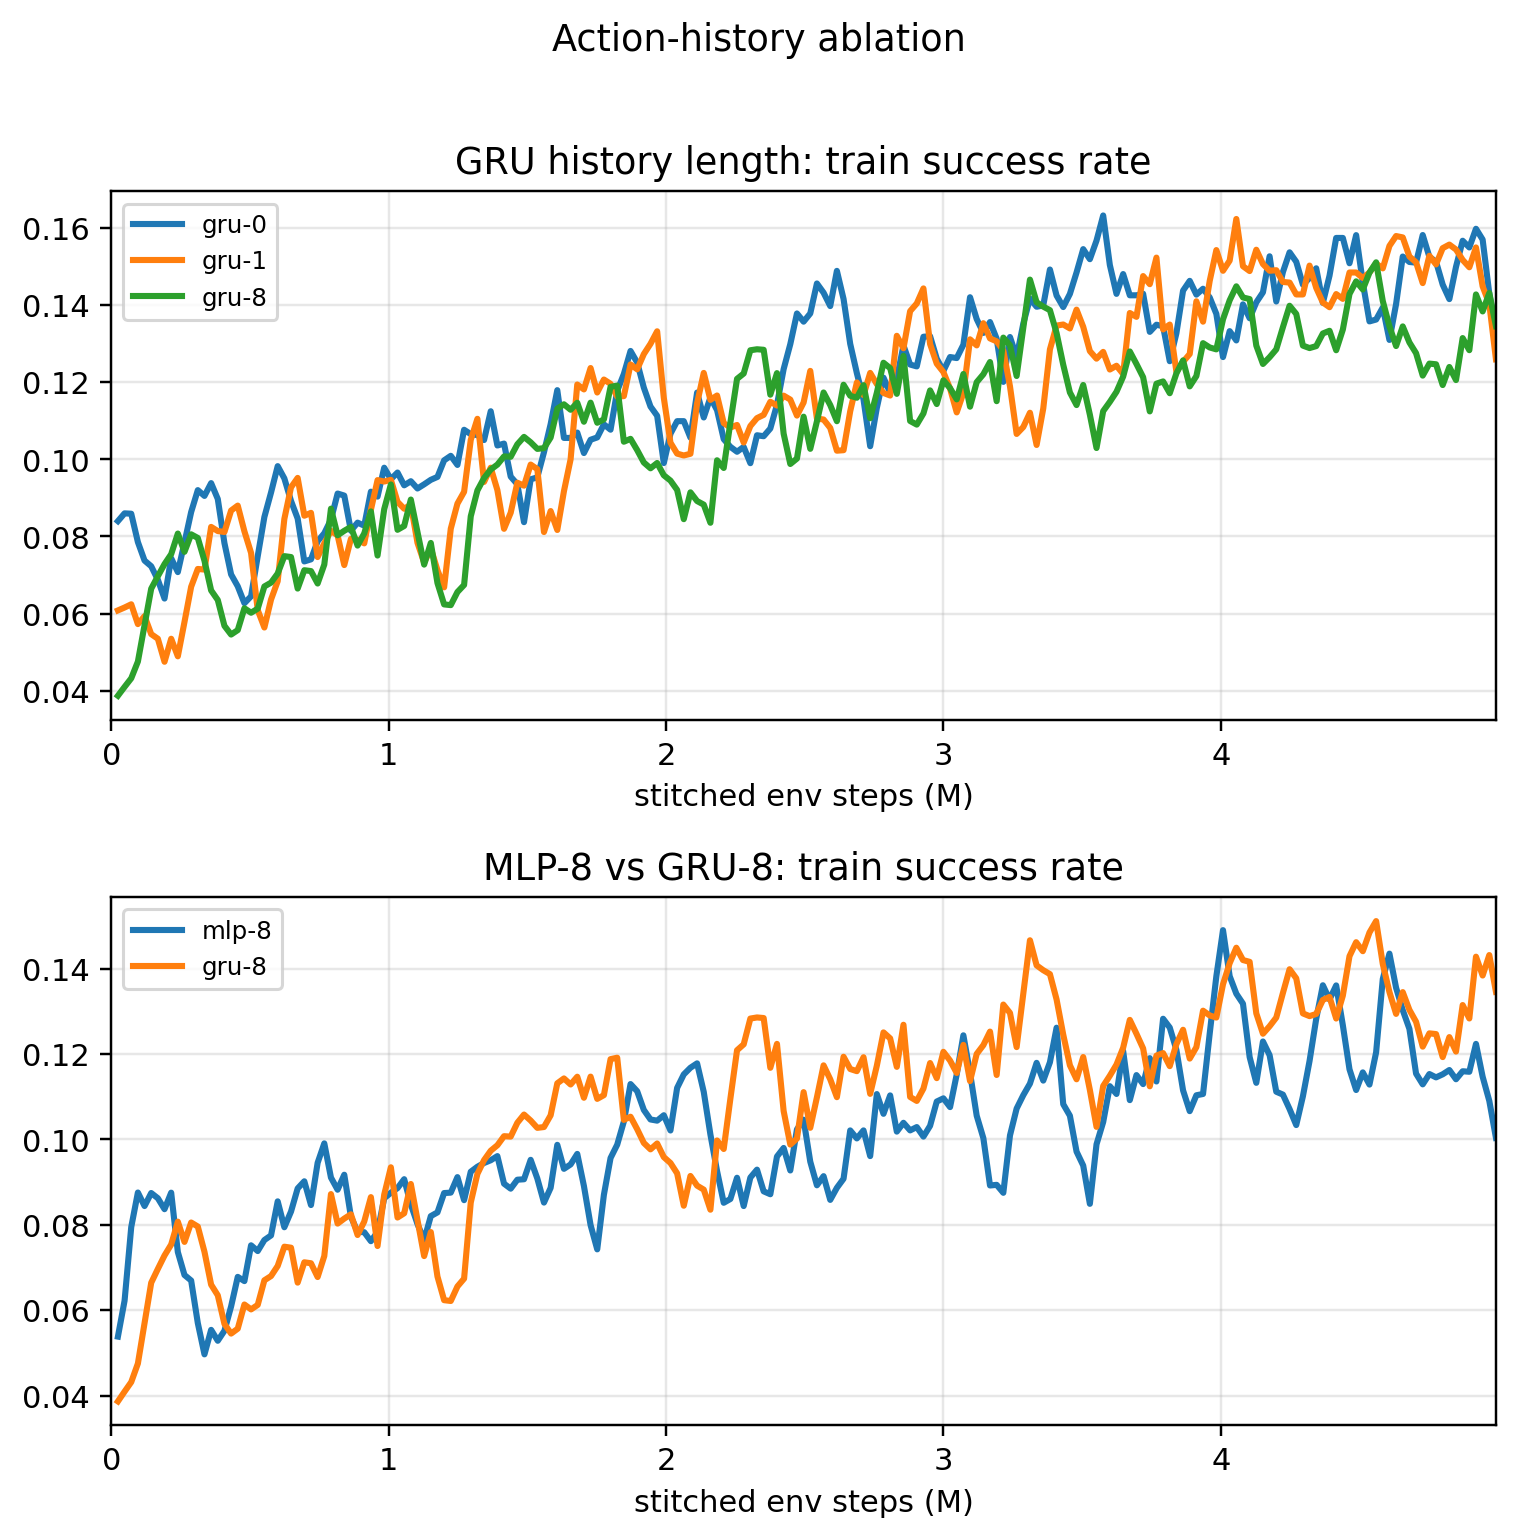
\includegraphics[width=\columnwidth]{figures/fig4_action_history_ablation.png}
\caption{动作历史长度消融。显式输入动作历史并不稳定优于无历史，\code{gru-8} 不及 \code{gru-0}，\code{mlp-8} 也劣于 \code{gru-8}；提升更可能来自 GRU 的时序建模能力，而非动作历史本身。}
\label{fig:history}
\end{figure}

\subsection{模型架构的影响}
图 \ref{fig:arch7x7} 与图 \ref{fig:history} 围绕原始 7x7 实验比较模型架构。结果显示，GRU 效果最好；显式输入动作历史会让 GRU 性能下降；\code{mlp-8} 比 \code{gru-8} 更差，CNN 在 7x7 小地图上则不占优。

对这一现象的解释口径如下：非 Markov 环境原则上可以通过把历史输入网络而被 Markov 化，因此从表示能力上并非完全做不到；但``可以表示''不等于``容易优化''，额外的历史输入会增大学习难度。因此 GRU 带来的提升更可能来自其时序建模能力本身，而不是来自动作历史这一额外输入。

\subsection{Credit assignment}
\label{sec:credit}
信用分配在 turn-based 设置下是真实且重要的问题。图 \ref{fig:credit} 给出 actor-side credit 在 \code{v1-nodl-nopush} 上的短程消融：几种 credit 项与主线大体重合，仅个别变体在 5M 末端有局部上冲，尚不足以支持稳定收益。当前结论是，active mask 是必要基础，而额外的 actor-side credit 收益有限。

\begin{figure}[!tbp]
\centering
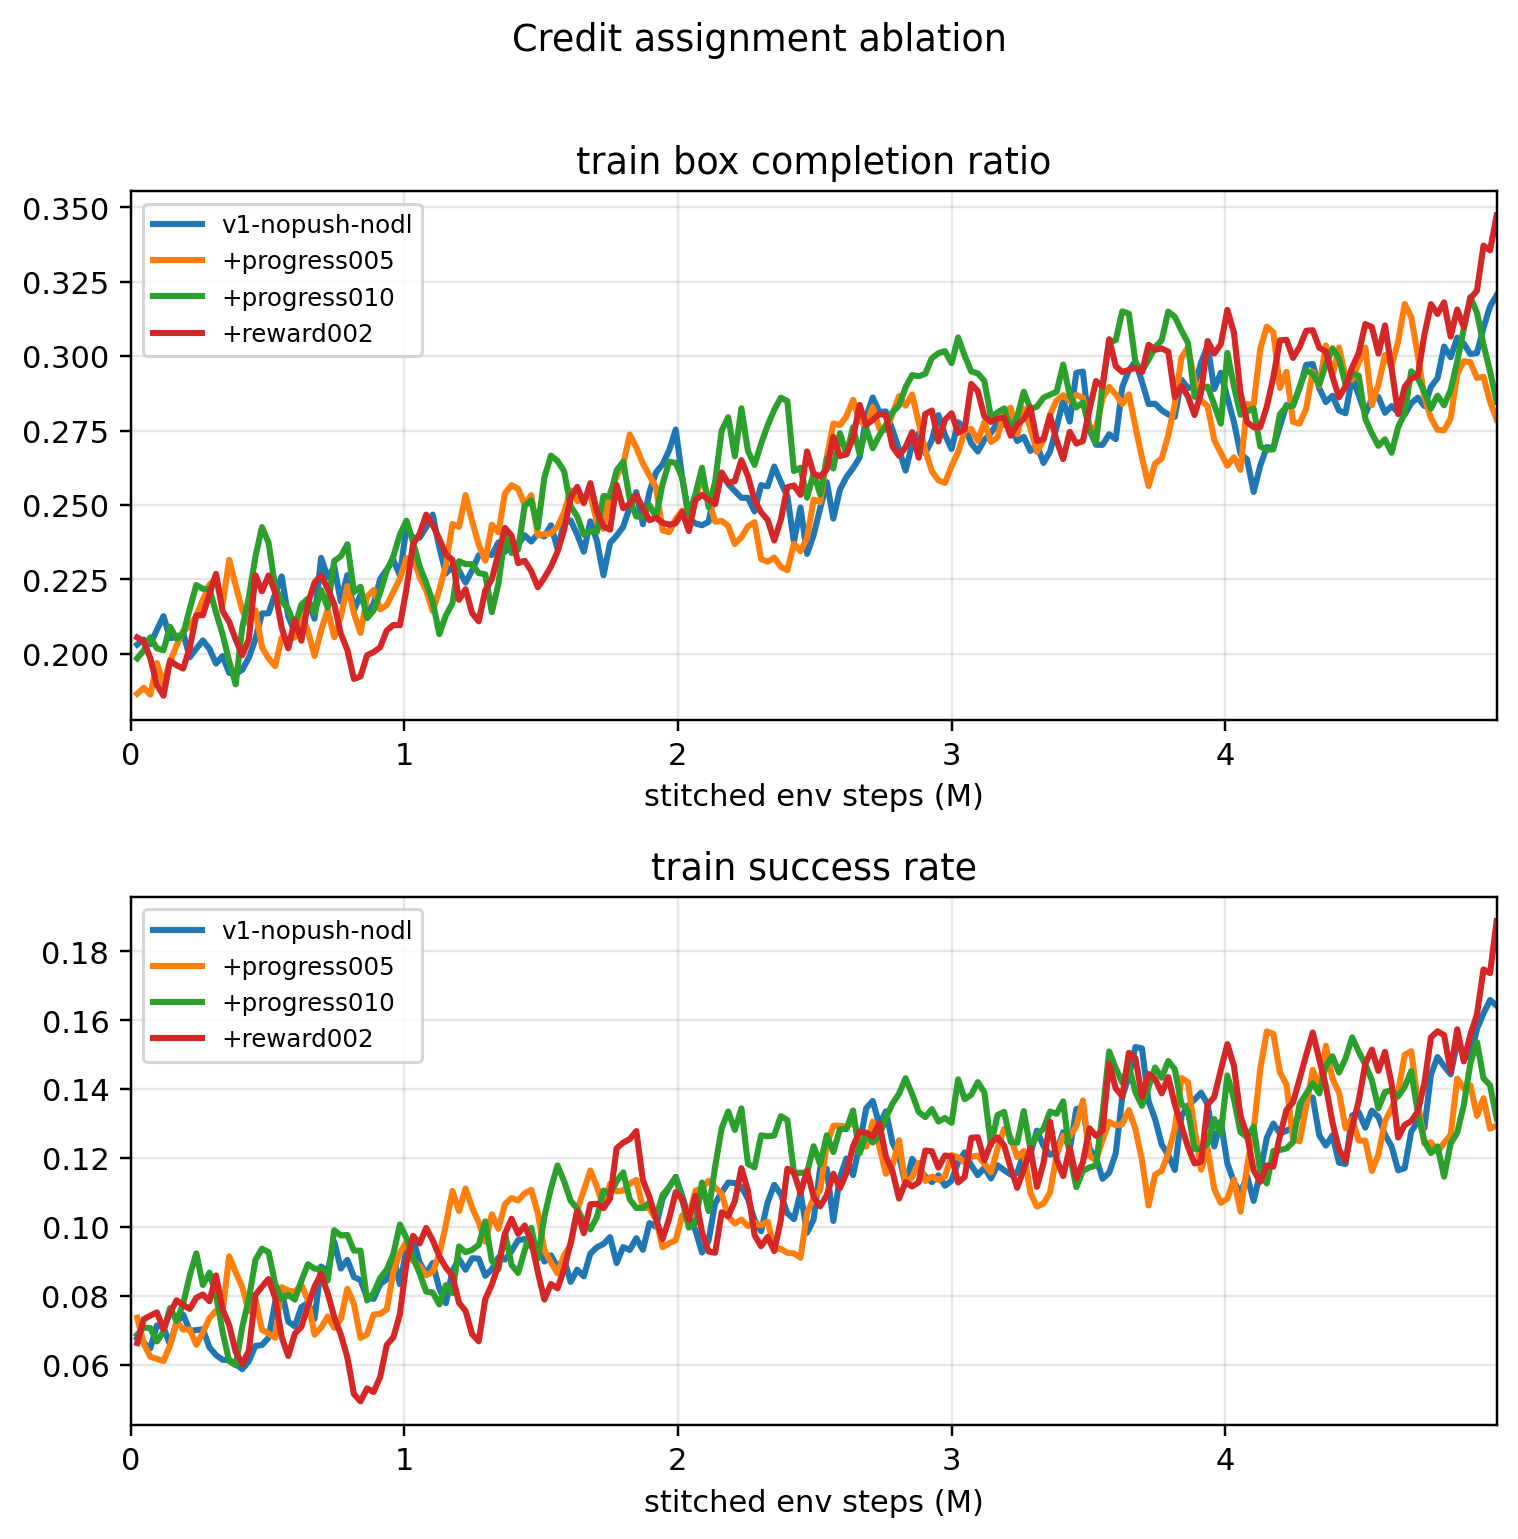
\includegraphics[width=\columnwidth]{figures/fig8_credit_assignment.png}
\caption{Actor-side credit 短程消融。各 credit 项与主线大体重合，5M 内仅有局部上冲，收益有限。}
\label{fig:credit}
\end{figure}

\subsection{HAHyPO}
\label{sec:hahypo}
图 \ref{fig:hahypo} 给出 HAHyPO 在 \code{v1-nodl-nopush} 上的 20M 对照。结果表明，引入 GRPO-style 优势并没有提升性能：小权重 $\alpha=0.2$ 基本跟随 HAPPO，$\alpha=0.5$ 明显偏弱，$\alpha=1.0$ 接近失败。其弱点在于轨迹级相对排序信号过粗，难以替代逐步 advantage。因此 HAHyPO 作为探索性方向可以保留，但不构成主线改进，也不应简单类比为``与语言模型一样有效''。

\begin{figure}[!tbp]
\centering
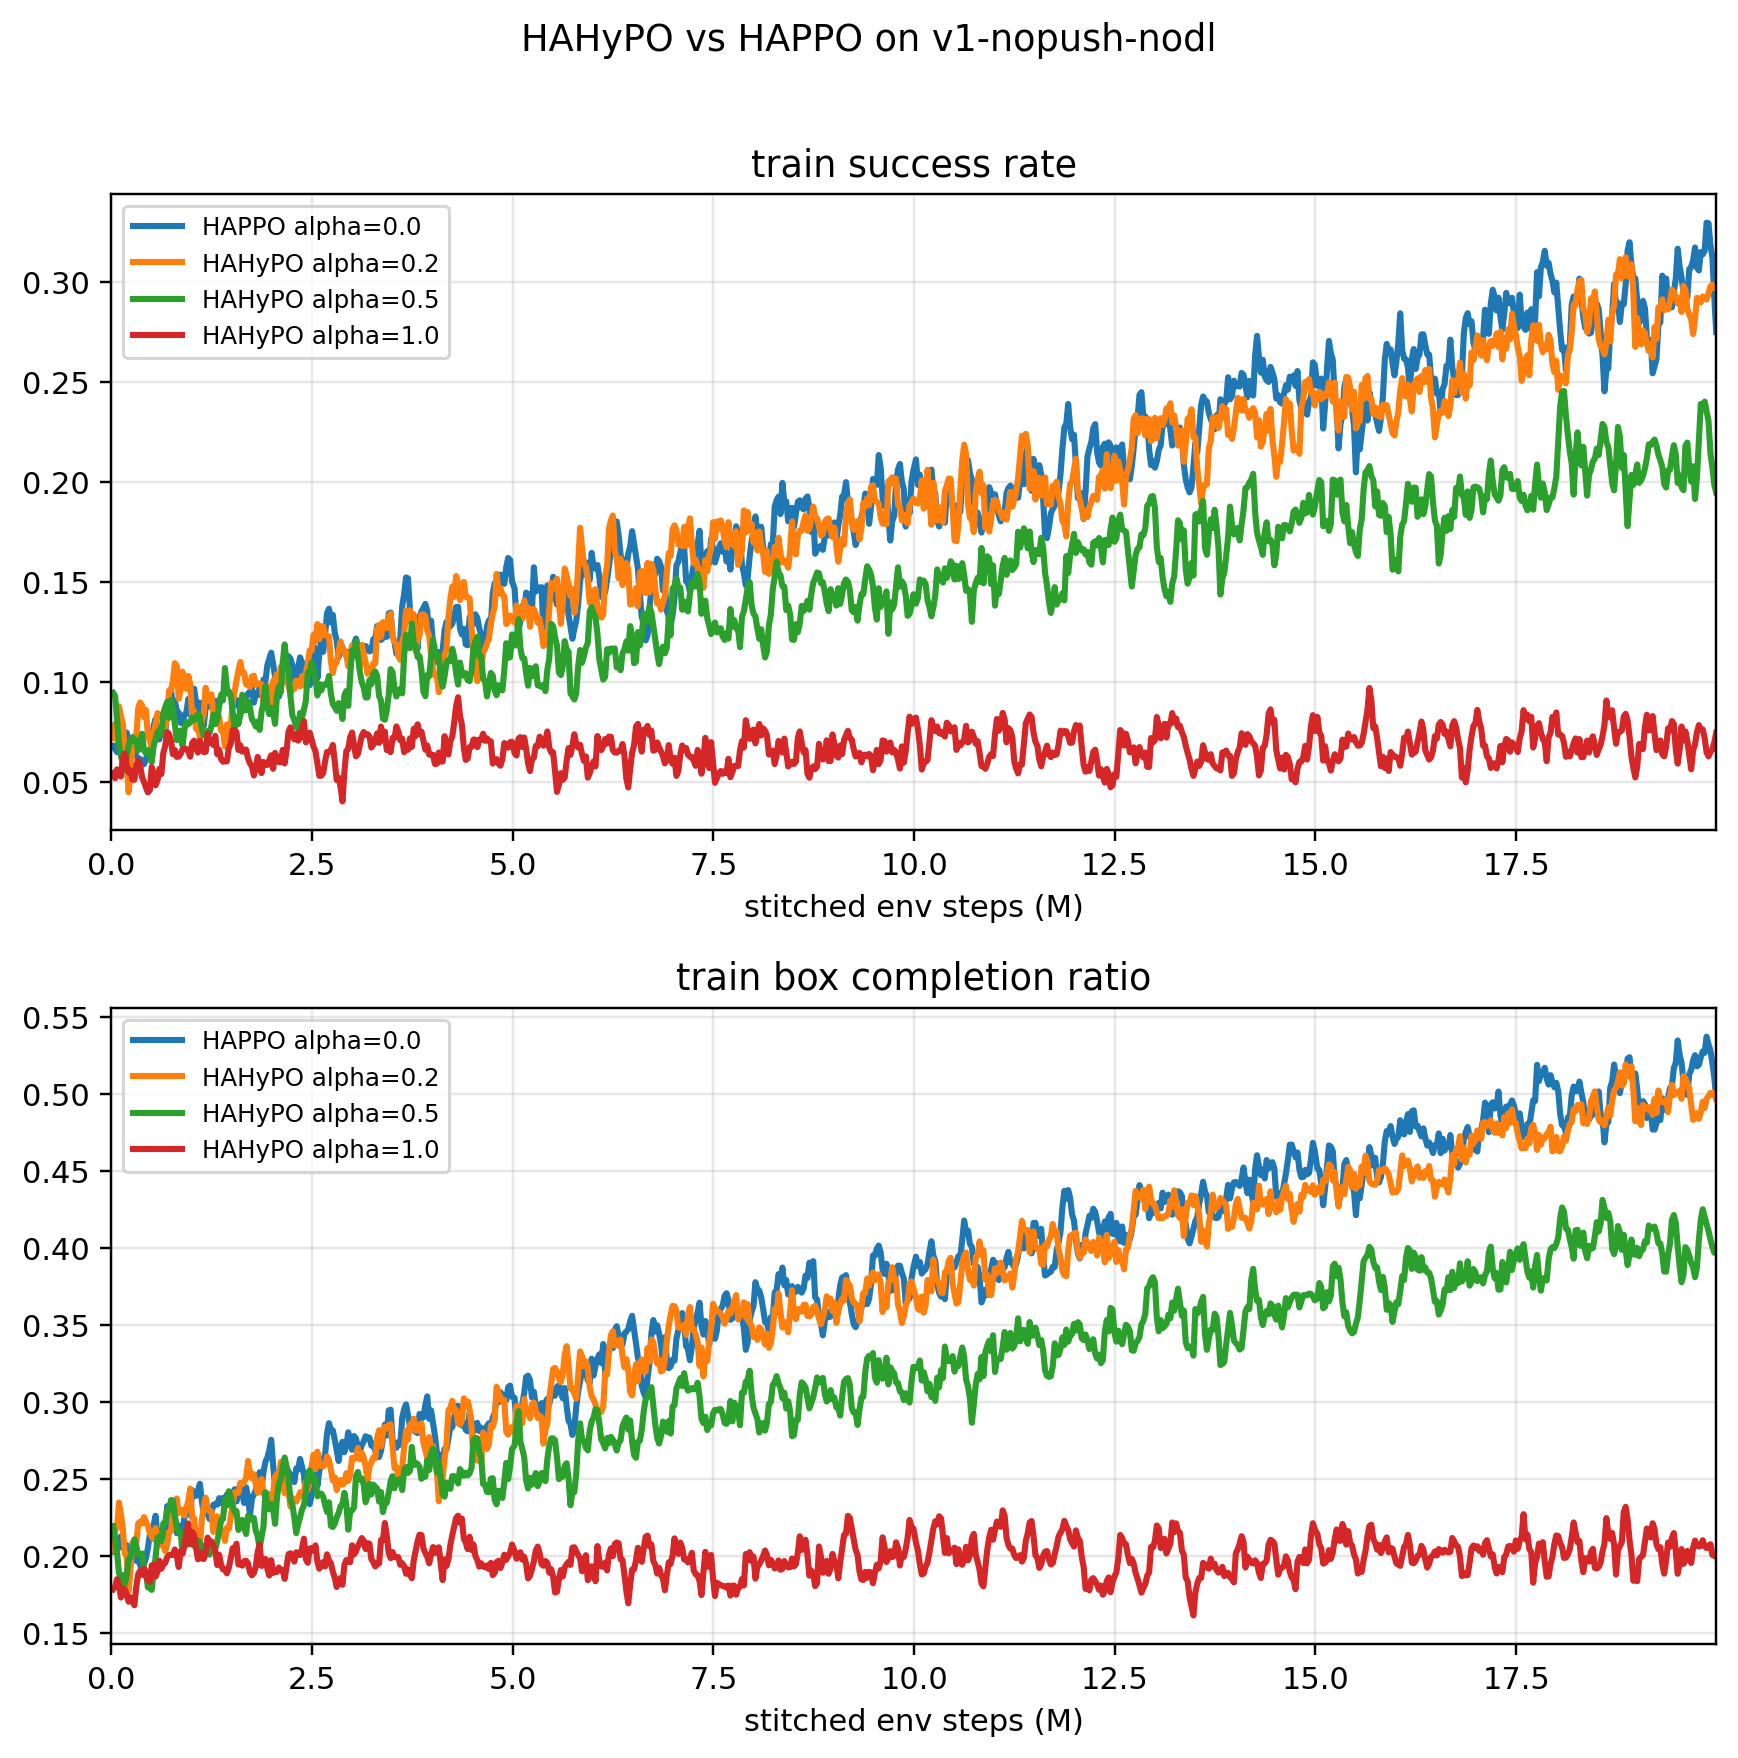
\includegraphics[width=\columnwidth]{figures/fig5_hahypo_vs_happo_v1.png}
\caption{HAHyPO 与 HAPPO 在 \code{v1-nodl-nopush} 上的比较。小权重 $\alpha=0.2$ 接近 HAPPO，$\alpha=1.0$ 明显破坏学习，GRPO-style 项未带来提升。}
\label{fig:hahypo}
\end{figure}



\subsection{Mix}
图 \ref{fig:random13} 与图 \ref{fig:topleft13} 展示了 13x13 兼容画布下的两种 padding。

\textbf{\code{random padding}} 几乎无法训练：有效信号稀疏，且模型需要在 7x7 的基础上额外学会平移不变性，到 20M 左右大多仍停留在低水平。

\begin{figure}[!tbp]
\centering
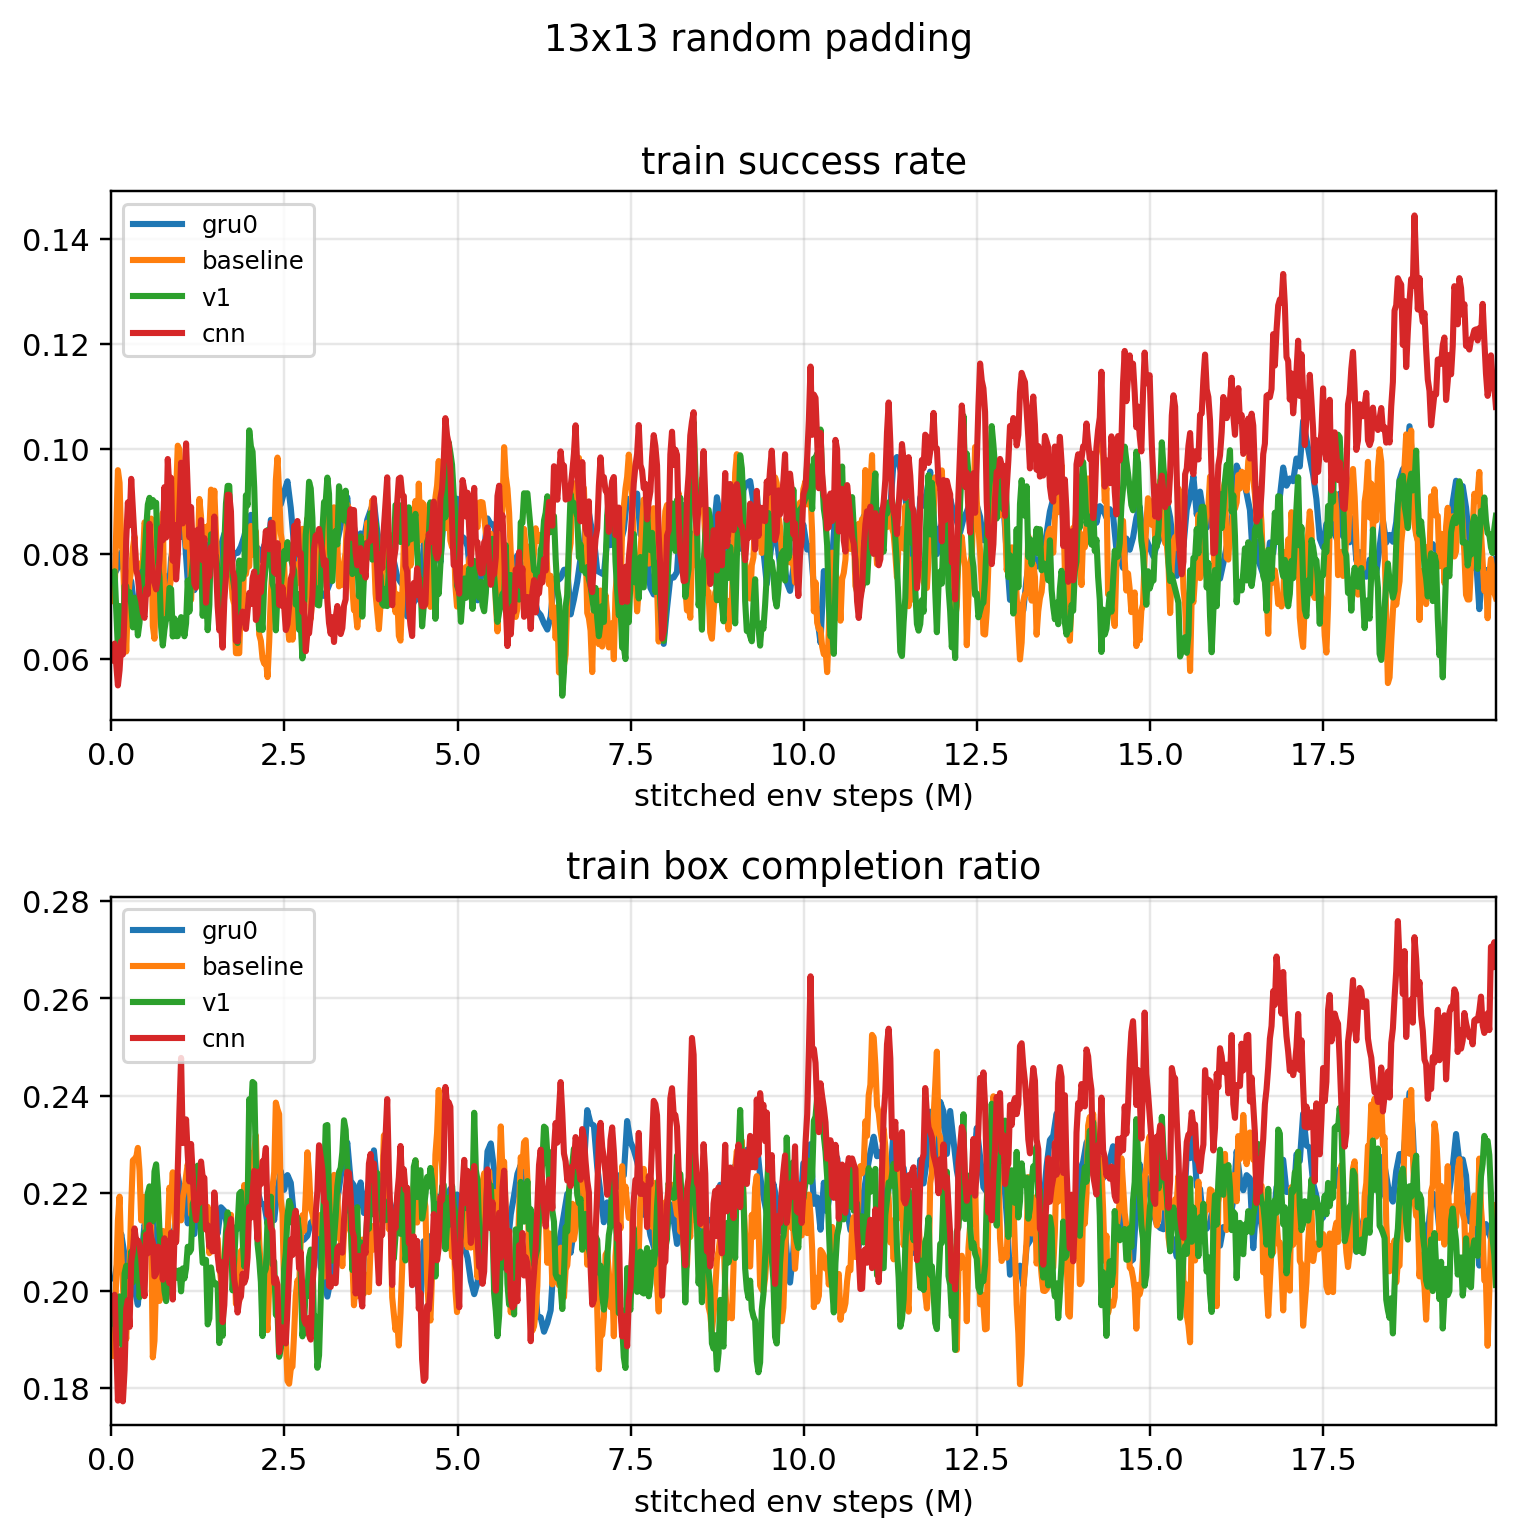
\includegraphics[width=\columnwidth]{figures/fig6_13random_train_metrics.png}
\caption{13x13 random padding 训练曲线。有效信号稀疏且需额外学会平移不变性，整体仍明显难于 7x7。}
\label{fig:random13}
\end{figure}

\textbf{\code{top-left padding}} 仍然困难，但 CNN 最优，其 train/eval success 与 eval box completion 都显著高于 MLP/GRU，这一结果显著体现了 CNN 的空间归纳偏置与平移不变性优势。一个值得强调的观察是：在原始等大输入实验中，曲线通常很快离开起始阶段，因此早期趋势对最终表现有较强指示；但在 13x13 top-left padding 中，训练会出现明显更长的平台期，random padding 的 warmup 平台可能更长。padding 并没有增加有效任务信息，只是扩大了观测维度和网络输入容量，模型仍需通过训练学会哪些位置是无信息的——对观察者而言，这相当于只能通过贝叶斯式的经验推断判断``某些输入区域不会带来信息''。因此，仅扩充输入规模或模型容量，即使不增加有效信息，也可能显著提高优化难度；容量提升通常需要与更丰富、更直接的训练信号匹配。这里只分析 20M 以内的平台期。

\begin{figure}[!tbp]
\centering
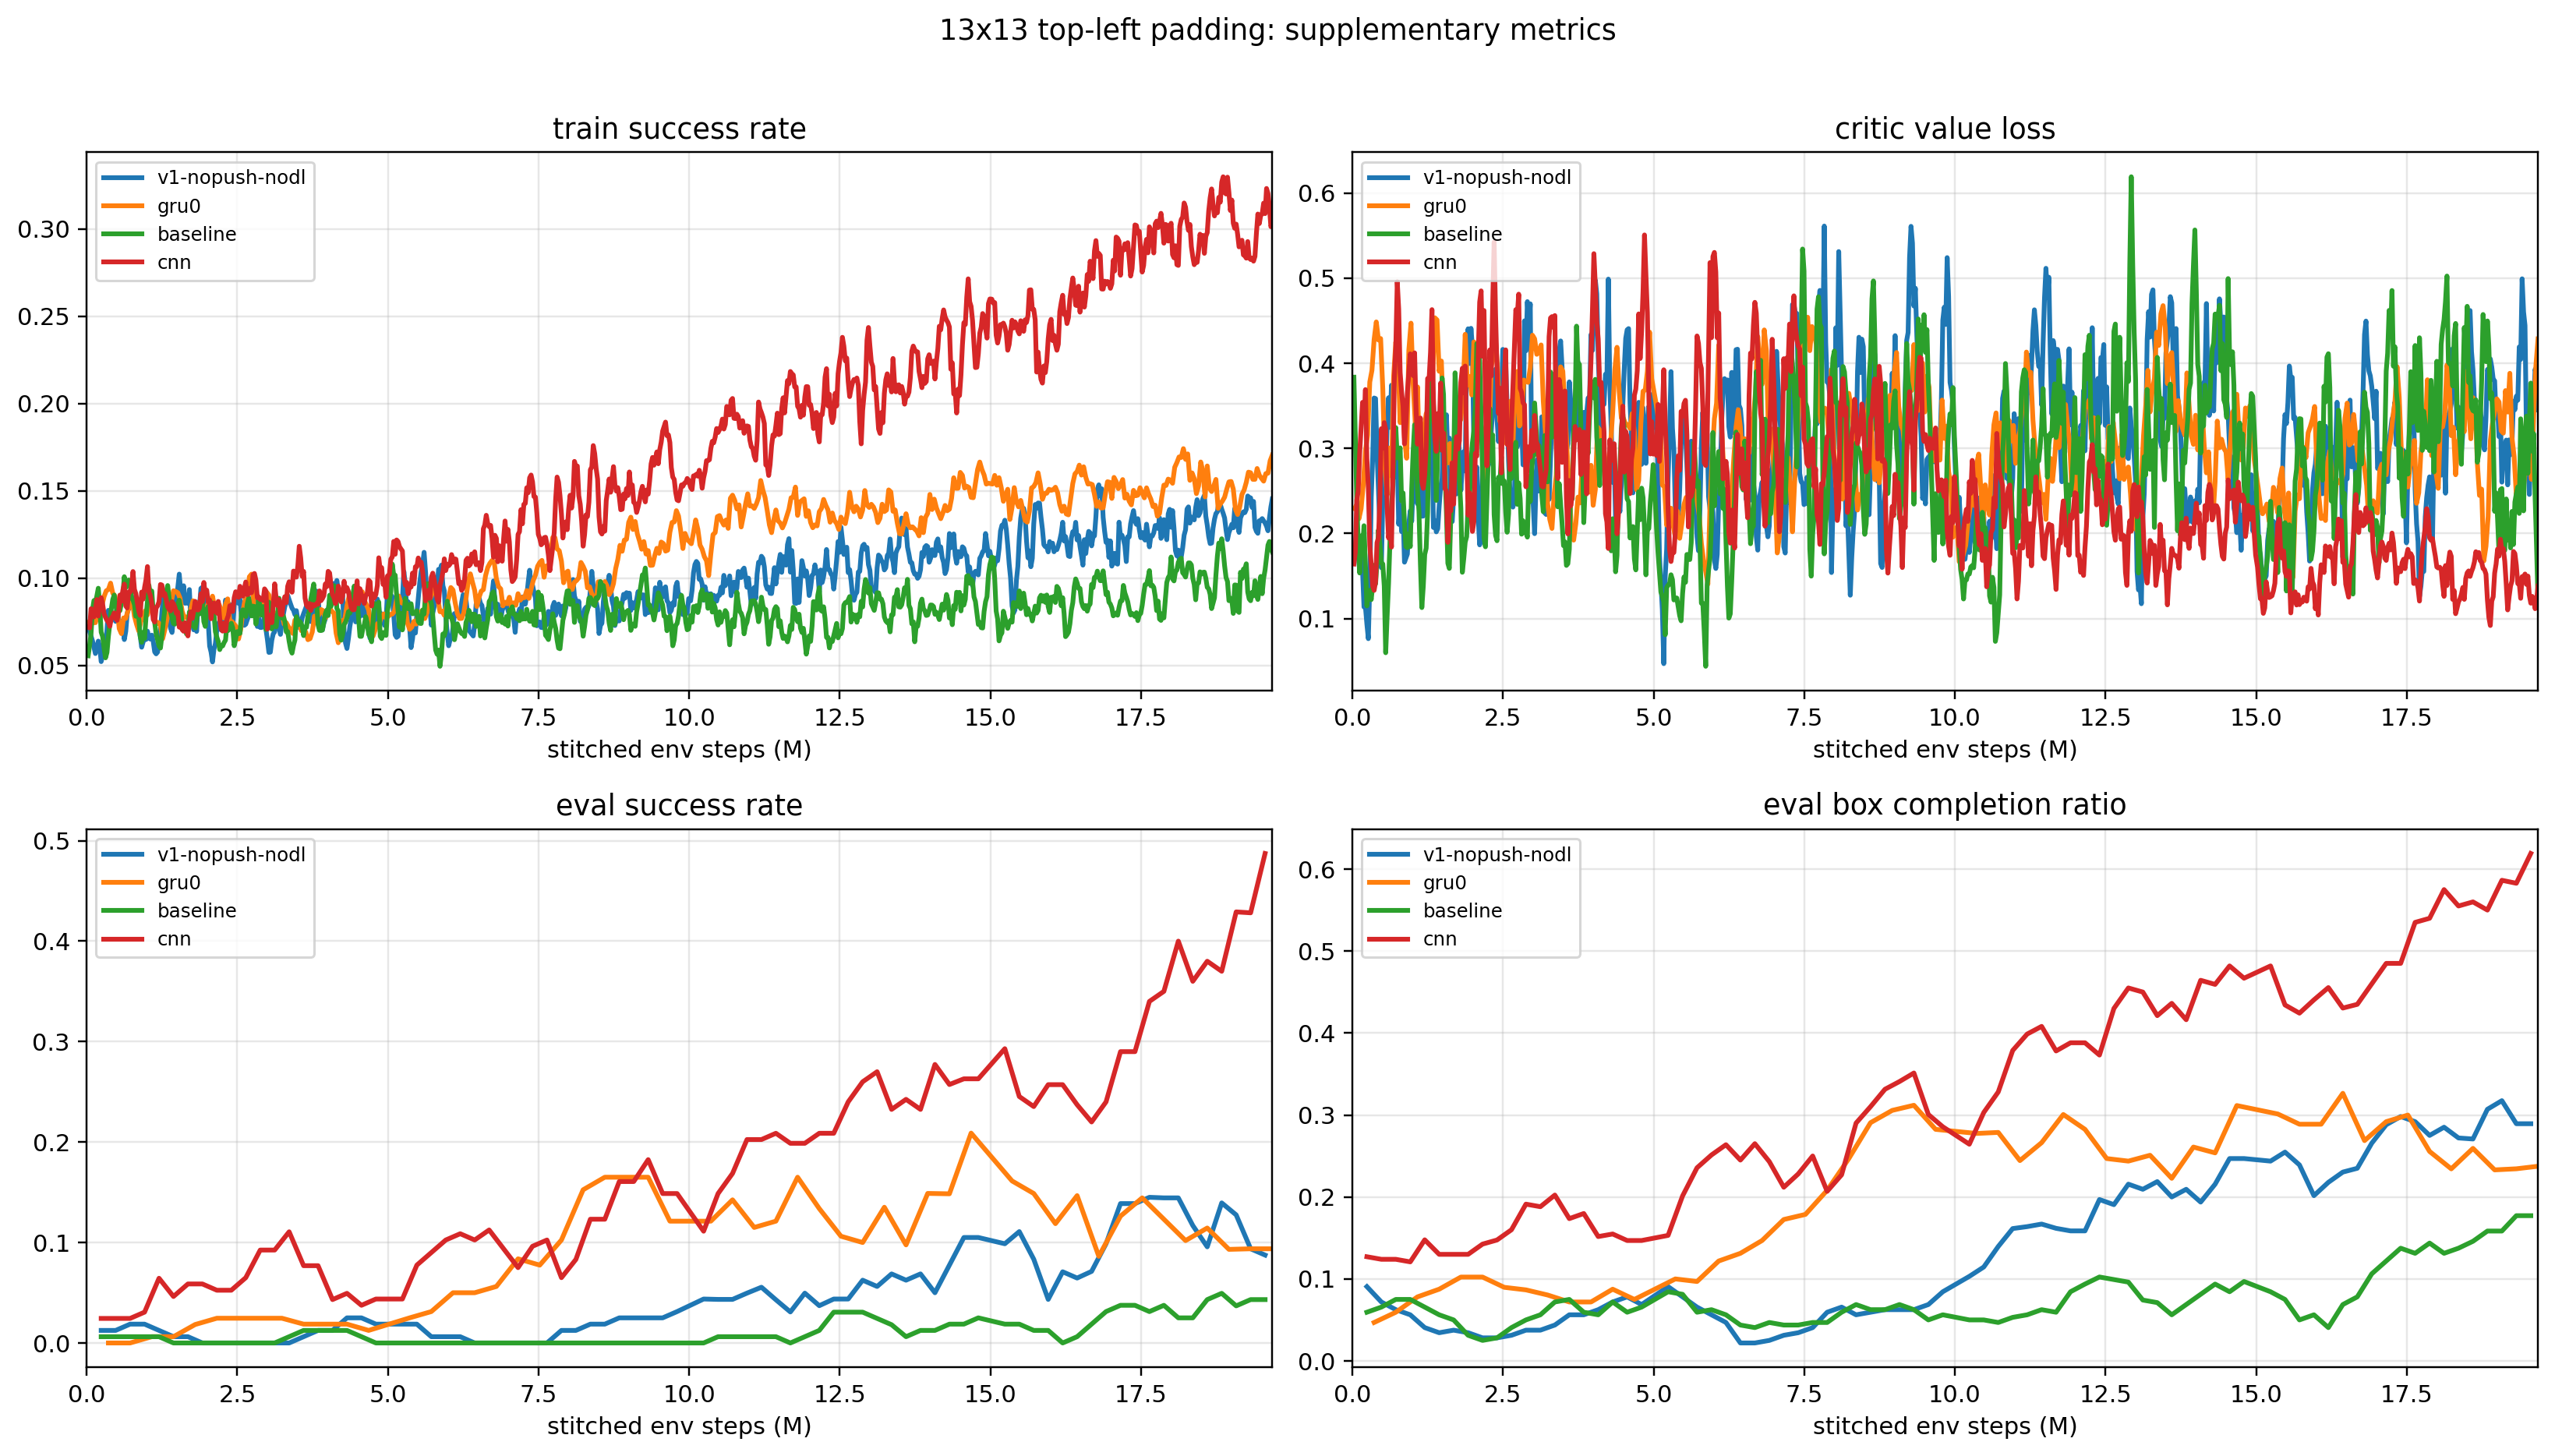
\includegraphics[width=\columnwidth]{figures/fig7_13tl_supp_metrics.png}
\caption{13x13 top-left padding 的补充指标。CNN 在固定对齐的大画布中明显优于 MLP/GRU，eval success 后期接近 0.5，eval box completion 超过 0.6，体现空间归纳偏置的价值。}
\label{fig:topleft13}
\end{figure}

我们还尝试把 7x7 长训策略 \code{distillation} 到 13x13 padded 模型。表 \ref{tab:distill} 与图 \ref{fig:distill} 显示，distillation 没有效果：\code{v1-nodl-nopush} distilled 模型在 20 个评估 episode 中仅成功 1 次，其余两组为 0。这很可能受限于模型容量，简单的行为克隆/蒸馏不足以跨越尺寸变化带来的表示错位。

\begin{table}[t]
\caption{13x13 distillation 后 20 个 episode 的评估均值。}
\label{tab:distill}
\centering
\begin{tabular}{lccc}
\toprule
模型 & 成功率 & 完成比例 & 平均回报 \\
\midrule
v1-noshape & 0.00 & 0.075 & -14.85 \\
v1-nodl-nopush & 0.05 & 0.125 & -12.93 \\
GRU-8action & 0.00 & 0.075 & -14.81 \\
\bottomrule
\end{tabular}
\end{table}

\begin{figure}[!tbp]
\centering
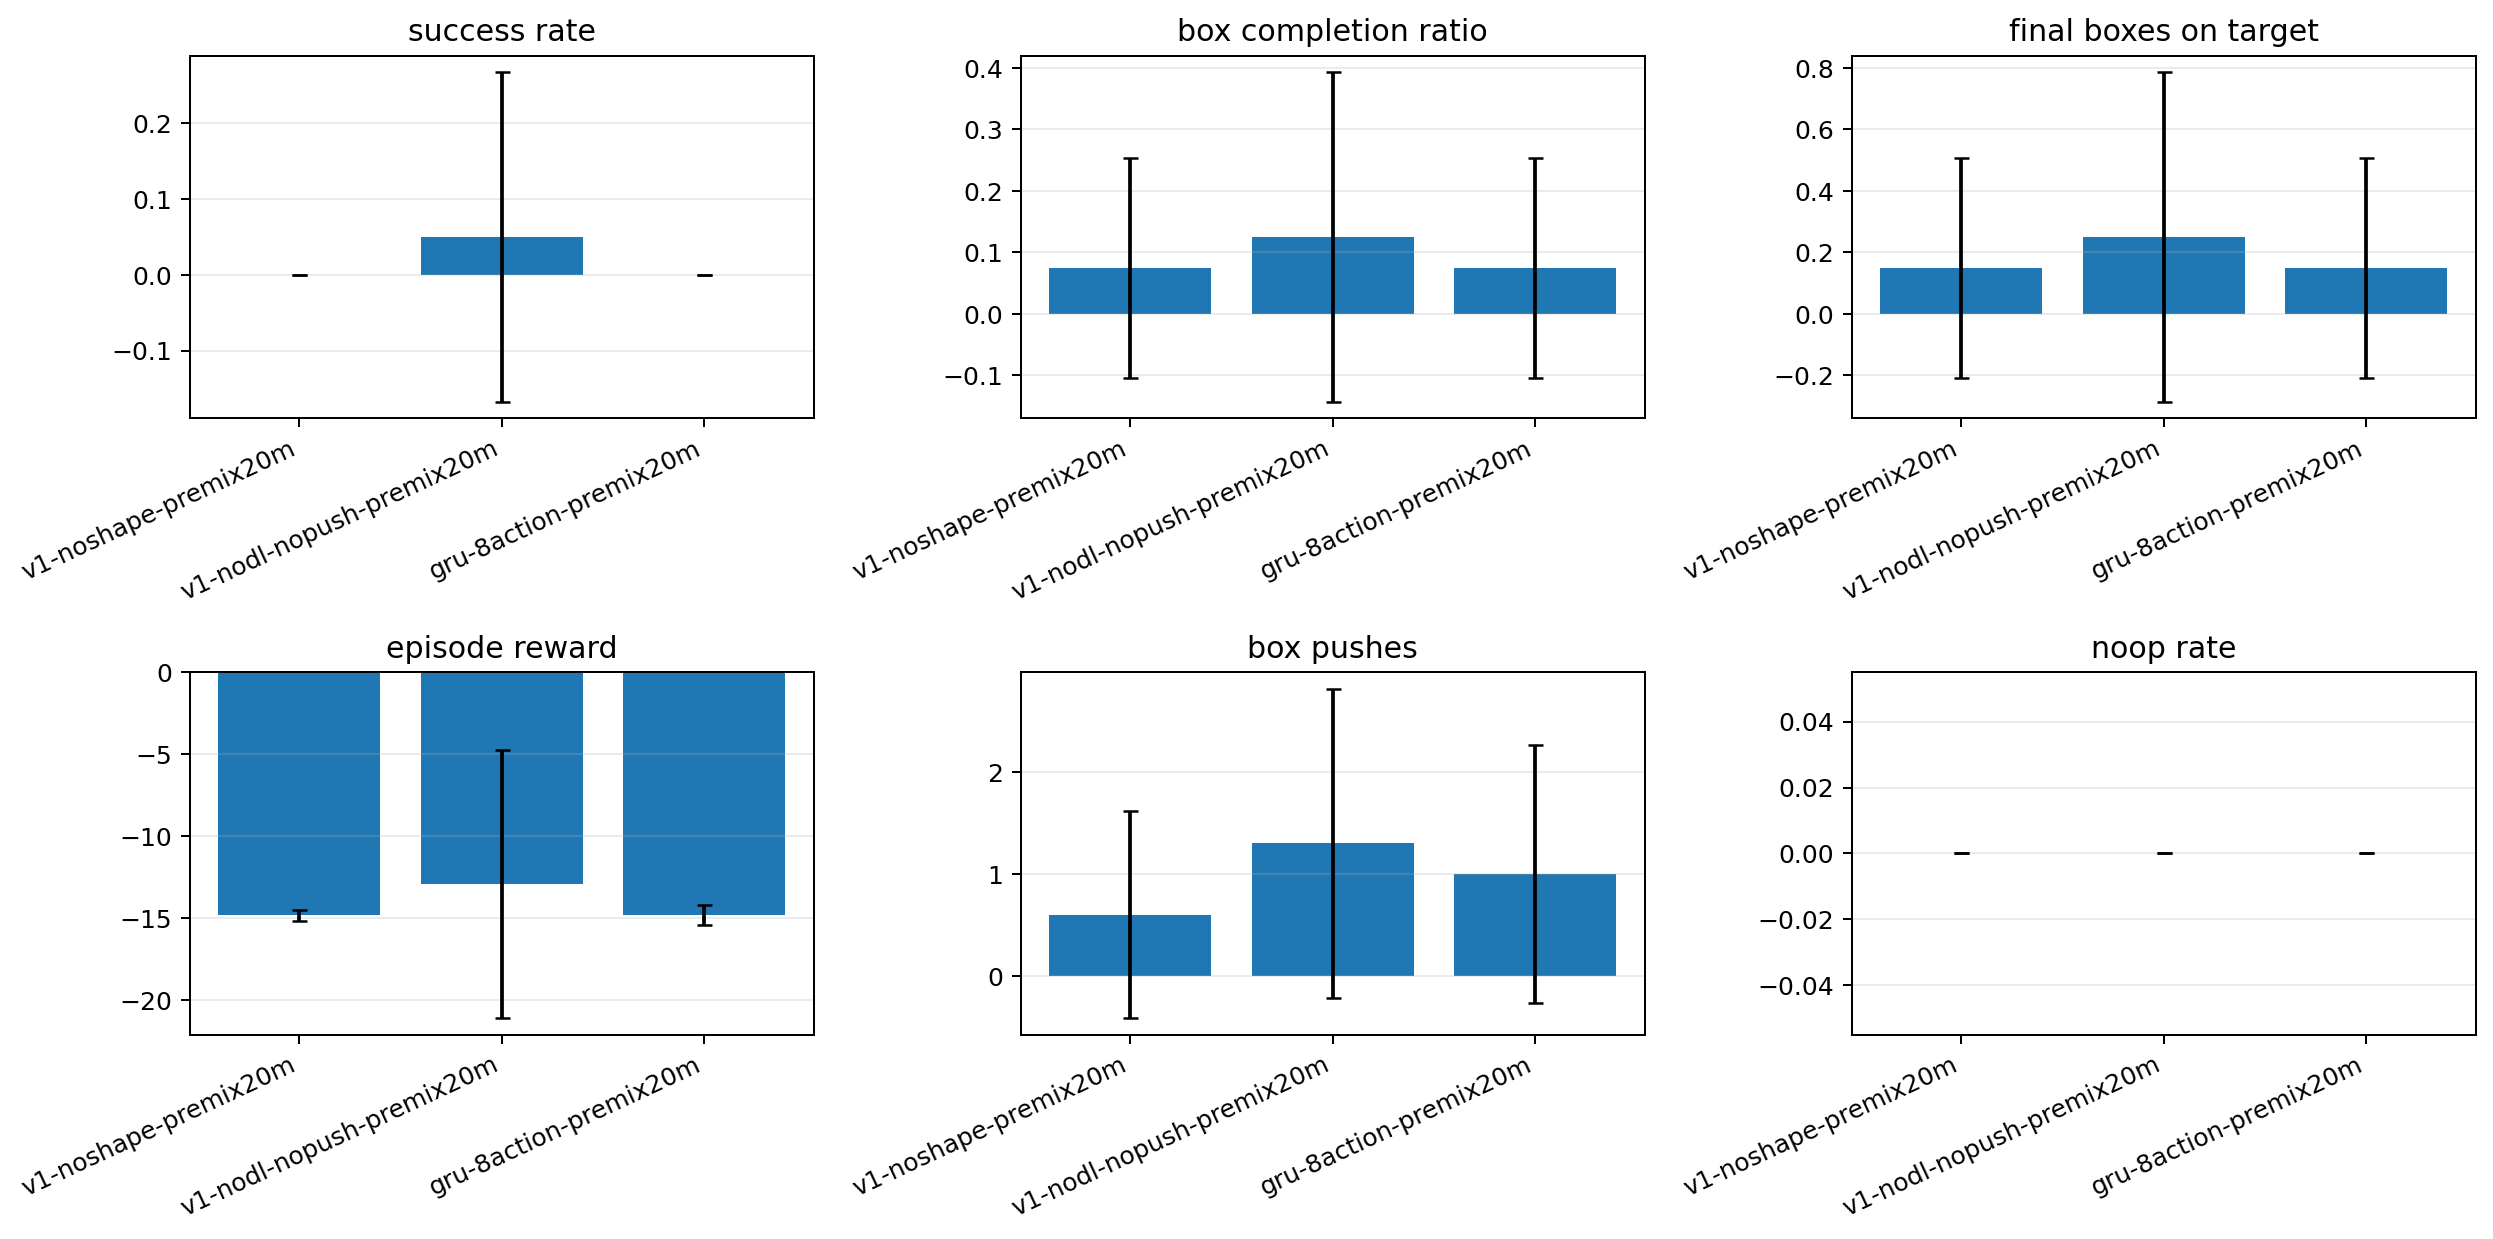
\includegraphics[width=\columnwidth]{figures/fig5_distill_eval_summary.png}
\caption{7x7 到 13x13 distillation 的评估统计。整体成功率很低，说明直接迁移无法可靠保留原策略能力，受限于模型容量。}
\label{fig:distill}
\end{figure}

\subsection{无用动作惩罚项}
作为行为先验的辅助分析，我们考察了无用动作惩罚项（对无效 push、撞墙移动、远离箱子时 \code{noop} 等施加小惩罚）。结果显示，该惩罚确实降低了 useless-action rate，并提高了 agent 的移动次数，说明奖励项改变了底层行为分布，使 agent 从``不动/浪费动作''转向更多行动。但其成功率与箱子到位率没有超过 \code{v1-nodl-nopush}，长程潜力反而较弱。这说明限制性能的主要因素并不是``没有合理动作''或``动作不够活跃''，而是推箱方向选择、长期规划与避免不可逆的错误 push。因此，无用动作惩罚验证了低层行为先验可以减少无效动作，但``多动''不等于会解 Sokoban，它应被理解为加速早期探索的行为先验，而非与任务完成直接相关的正向信号。

\section{结论与启发}
综合现有材料，我们得到以下结论：
\begin{enumerate}[leftmargin=1.4em,itemsep=0.25em]
    \item 主结果：HAPPO 在 7x7、2 boxes 下可以稳定学到协作策略；保留正向势函数、去掉 deadlock 与 pushability 负项的 \code{v1-nodl-nopush} 是当前实现中最稳的 baseline。
    \item 距离语义：更符合推箱语义的 reverse-push v2 并未带来更高成功率，更精确的 reward 反而使优化更崎岖；不可达距离的 cap 对控制信号尺度十分关键。
    \item 模型架构：GRU 表现最好，显式动作历史会降低 GRU 性能，\code{mlp-8} 也劣于 \code{gru-8}；历史输入虽能在原理上把环境 Markov 化，但``可表示''不等于``易优化''，CNN 在 7x7 不占优。
    \item 信用分配：turn-based active mask 是必要基础，但当前 actor-side credit 收益有限。
    \item HAHyPO：引入 GRPO-style 优势没有提升性能，其轨迹级相对排序信号过粗，难以替代逐步 advantage；可作为探索性方向保留，不构成主线改进。
    \item Mix：13x13 random padding 几乎无法训练，top-left padding 虽仍困难但 CNN 明显最优，体现了空间归纳偏置与平移不变性的价值；distillation 受限于模型容量而未见效果。若追求泛化，应优先使用更强空间归纳偏置与课程学习，而不是单点调 reward。
\end{enumerate}

\section{复现说明}
第一次配置环境可运行：
\begin{lstlisting}[language=bash]
cd /path/to/MARL-project-Sokoban
ENV_NAME=harl-sokoban TORCH_CHANNEL=cu118 \
  bash HARL/scripts/setup_sokoban_linux.sh
conda activate harl-sokoban
python HARL/scripts/verify_sokoban_setup.py
\end{lstlisting}
主线 7x7 实验入口示例：
\begin{lstlisting}[language=bash]
bash run6.2.sh                 # v1-nodl-nopush first 5M
bash run8/run_general8.3.sh    # continue + mix pipeline
bash run9/run_general9.1.sh    # GRU/action-history pipeline
bash run15/run_general15.1_top_left13_curriculum_all.sh
\end{lstlisting}
图表生成脚本位于 \path{HARL/scripts/plot_report_key_metrics.py}、\path{HARL/scripts/plot_report_ablation_figures.py}、\path{HARL/scripts/plot_v2_cap12_full_comparison.py} 和 \path{HARL/scripts/eval_distilled_sokoban.py}。

\section{最优模型}
最终提交模型确定为 \code{GRU0}，即采用 GRU encoder、不显式输入动作历史的版本。其设置如下：
\begin{itemize}[leftmargin=1.2em,itemsep=0.2em]
    \item 环境设置：7x7 Sokoban，2 boxes，\code{TwoPlayer-Sokoban-v0}，\code{max_steps=150}。
    \item reward shaping：\code{v1-nodl-nopush} BFS 势函数，保留 box-target 与 agent-box 正向势（$w_{bt}=0.20$、$w_{ab}=0.10$），去掉 deadlock 与 pushability 负项，\code{reward_finished=20}。
    \item 架构与历史长度：GRU encoder，动作历史长度为 0。
    \item 训练步数：经多阶段续训累计约 40M stitched steps。
    \item 选用理由：\code{GRU0} 在 7x7 主线中整体更稳，且不引入动作历史带来的额外优化负担，这与正文模型架构结论一致。
\end{itemize}

评测指标方面，\code{GRU0} 在约 40M steps 后的最后一次 raw evaluation 中达到 eval success rate $=1.00$、box completion ratio $=1.00$；报告图像经过 smoothing，视觉上可能低于该 raw 点，最近 10 次 evaluation 的平均 success rate 约 0.72、box completion ratio 约 0.81。最终 checkpoint 整理在仓库根目录 \path{finalmodel/} 下（含 \code{models/}、\code{config.json} 与独立脚本 \code{eval_finalmodel.py}）；运行该脚本即可在 v0 环境复测，加 \code{--scenario_pool config} 则做 v0/v1/v2 混合 deterministic 评测（一次 30-episode mixed re-eval 的 overall success rate 为 0.60、box completion ratio 为 0.75）。引用时需写清 v0-only 或 mixed-scenario 口径。

\section*{致谢}
本项目基于 \code{gym-sokoban} 环境和 PKU-MARL HARL 框架实现，课程作业要求提供了 HAPPO 等多智能体强化学习基准方向。

\bibliography{references}
\bibliographystyle{icml2022}

\end{document}
